\documentclass[12pt,a4paper]{article}
\usepackage[utf8]{inputenc} %polskie znaki
\usepackage[T1]{fontenc}	%polskie znaki
\usepackage{amsmath}		%matematyczne znaczki :3
\usepackage{enumerate}		%Dodatkowe opcje do funkcji enumerate
\usepackage{geometry} 		%Ustawianie marginesow
\usepackage{graphicx}		%Grafika
\usepackage{wrapfig}		%Grafika obok textu
\usepackage{float}			%Allows H in figure
\usepackage{hyperref}		%Allows hyperlinks
%\pagestyle{empty} 			%usuwa nr strony
\usepackage{todonotes}		%Todo notatki
\usepackage{lipsum}         %Lorem text
\usepackage{ntheorem}   	% for theorem-like environments
\usepackage{mdframed}   	% for framing
\usepackage{subcaption}		% subfigure (image placing)
\usepackage{pdfcomment}		% Komentarze (z bazowego pdf'a)
\usepackage{xparse}			% New commands with optional arguments
\usepackage{ifthen}			% If then - funkcje!
\usepackage{expl3}			% Deklarowanie zmiennych
\usepackage{pgf}			% Aktualne rachunki \pgfmathparse{}
\usepackage{amsmath} 		% For mathematical symbols and structures
\usepackage{amsfonts}		% Zbiór liczb naturalnych + formatowanie
\usepackage{ulem}			% Przekreślony text
%\usepackage[colorlinks=true, linkcolor=blue, urlcolor=red, citecolor=green]{hyperref}
\usepackage{fontawesome5}
\usepackage{mathtools}

\newgeometry{tmargin=2cm, bmargin=2cm, lmargin=2cm, rmargin=2cm} 

%Counter commands{
	\newcounter{definicja}
	\setcounter{definicja}{1} 
	\newcounter{twierdzenie}
	\setcounter{twierdzenie}{1} 
	\newcounter{przyklady}
	\setcounter{przyklady}{1} 
	\newcounter{wnioski}
	\setcounter{wnioski}{1} 
	
	\newcommand{\counter}[1]{
		\arabic{#1} \stepcounter{#1} 
	}
	\newcommand{\counterreset}[1]{\setcounter{#1}{1}}
	%}

%Define styles{
	\theoremstyle{break}
	\theoreminframepreskip{0.5cm}
	\theoremheaderfont{\bfseries}
	\newmdtheoremenv[%
	linecolor=white,%
	innertopmargin=\topskip,
	shadowsize=0,%
	innertopmargin=5,%
	innerbottommargin=5,%
	leftmargin=10,%
	rightmargin=10,%
	backgroundcolor=gray!20,%
	innertopmargin=0pt,%
	ntheorem]{zad}{Zadanie}
	
	\mdfdefinestyle{zadanie}{
		linecolor=white,%
		innertopmargin=5,%
		innerbottommargin=5,%
		leftmargin=10,%
		rightmargin=10,%
		backgroundcolor=gray!20,%
		innertopmargin=8,
		innerbottommargin=8,
		skipabove = 5,
	}
	\mdfdefinestyle{wzor}{
		linecolor=cyan,%
		linewidth=2pt,%
		innertopmargin=8,
		innerbottommargin=8,
		leftmargin=10,%
		rightmargin=10,%
		backgroundcolor = white, 
		fontcolor = black,
		skipabove = 5,
		skipbelow = 5,
	}
	%}

%Zadania templatex%{
	\newcommand{\Obramowka}[1]{
		\begin{mdframed}[style=wzor]
			\centering #1
		\end{mdframed}
	}
	\newcommand{\Komentarz}[1]{
	\begin{mdframed}[style=zadanie]
		\textbf{Komentarz}\\
		#1
	\end{mdframed}
	}
	
	%}

% Set spacing before and after theorems
\setlength{\theorempreskipamount}{20pt}  % Space above the theorem
\setlength{\theorempostskipamount}{20pt} % Space below the theorem

\newtheorem{definition}{Definicja}[section]

\newtheorem{theorem}{Twierdzenie}[section]
\newtheorem{lemma}{Lemat}[section]
\newtheorem{wniosek}{Wniosek}[theorem]
\newtheorem{example}{Przykład}[section]
\newtheorem{exercise}{Ćwiczenie}[section]
\newtheorem{stwierdzenie}{Stwierdzenie}[section]
\newtheorem{obserwacja}{Obserwacja}[section]


\newcommand{\tg}{\text{tg}}
\newcommand{\ctg}{\text{ctg}}
\newcommand{\witw}{$\Leftrightarrow$}
\newcommand{\wynika}{$\Rightarrow$}
\newcommand{\UkladRownan}[2]{
	$\left\{
	\begin{array}{l}
		#1 \\
		#2
	\end{array}
	\right.$
}

\begin{document}
	% Strona tytułowa
	
	% Dodanie strony tytułowej
	\begin{titlepage}
		\centering
		\vspace{1cm}
		{\Huge\bfseries Matematyczne aspekty wyborów \par} 
		\vspace{1.5cm}
		{\large Na podstawie wykładu \par} 
		\vspace{0.5cm}
		{\Large Krzysztofa Ciesielskiego}\\
		\vspace{1cm}
		{\large Skrypt autorstwa}\\
		\vspace{0.5cm}
		{\Large Arkadiusza Dąbala}\\
		\vfill 
		{\large Wersja z dnia:}\\
		{\Large \today \par}  
		\vspace*{1cm}
	\end{titlepage}
	\newpage
	\tableofcontents
	\newpage
\section{Preliminaria}
\subsection{Jak wyglądają aktualnie wybory?}
\Komentarz{Materiał ten nie ma w żadnym stopniu charakteru politycznego, a wyłącznie charakter matematyczny.}

\begin{example}
Rozważmy poniższe dane, oparte na 6 partiach, 1000 głosach i 6 mandatów do rozdania:
\end{example}

\begin{tabular}{|c|c|c|c|c|c|c|}\hline
	Nazwa        & Głosy & $:1$ & $:2$ & $:3$ & $:4$ & Otrzymane mandaty\\\hline
	Filateliści  & 380   & \textbf{380} & \textbf{190} & \textbf{127} & 87   & 3\\\hline
	Gitarzyści   & 192   & \textbf{192} & \textbf{96}  & 64   &       & 2\\\hline
	Szachiści    & 180   & \textbf{180} & 90    &       &       & 1\\\hline
	Piłkarze     & 96    & \textbf{96}  & 48    &       &       & 1\\\hline
	Lotniarze    & 90    & 90    &       &       &       & 0\\\hline
	Kolejarze    & 62    & 62    &       &       &       & 0\\\hline
\end{tabular}\\

System ten działa w następujący sposób:

\begin{itemize}
	\item Liczby głosów dzielone są przez kolejne liczby naturalne dodatnie (tak jak w tabeli).
	\item Wybierane są z tej tabeli 6 największych liczb (wytłuszczony druk).
	\item Liczba mandatów zależy od liczby wytłuszczonych liczb w wierszu partii.
\end{itemize}

\begin{example}
	Rozważmy tę samą tabelę, ale załóżmy, że partia \textbf{Gitarzyści} nie przekroczyła progu $5\%$.
\end{example}

\begin{tabular}{|c|c|c|c|c|c|c|}\hline
	Nazwa        & Głosy & $:1$ & $:2$ & $:3$ & $:4$ & Otrzymane mandaty\\\hline
	Filateliści  & 380   & \textbf{380} & \textbf{190} & \textbf{127} & 87   & 3\\\hline
	\sout{Gitarzyści}  & \sout{192}  & \sout{192} & \sout{96}  & \sout{64}  & \sout{---} & \sout{---} \\\hline
	Szachiści    & 180   & \textbf{180} & \textbf{90}  &       &       & 2\\\hline
	Piłkarze     & 96    & \textbf{96}  & 48    &       &       & 1\\\hline
	Lotniarze    & 90    & \textbf{90}  &       &       &       & 1\\\hline
	Kolejarze    & 62    & 62    &       &       &       & 0\\\hline
\end{tabular}\\

\begin{example}
	Rozważmy następującą tabelę z 5 mandatami do rozdania:
\end{example}

\begin{tabular}{|c|c|c|c|c|c|}\hline
	Nazwa    & Głosy $:1$ & $:2$ & $:3$ & $:4$ & Mandaty\\\hline
	Rybacy   & \textbf{6000} & \textbf{3000} & \textbf{2000} & 1500 & 3\\\hline
	Myśliwi  & \textbf{5700} & \textbf{2850} & 1900  &       & 2\\\hline
	Artyści  & 1950          & 975           &       &       & 0\\\hline
\end{tabular}\\

Partia \textbf{Rybacy} prowadziła kampanię przeciwko \textbf{Myśliwym}, w wyniku czego liczba otrzymanych głosów zmieniła się następująco:
\begin{itemize}
	\item Partia \textbf{Rybacy} zyskała 400 głosów (+400)
	\item Partia \textbf{Myśliwi} straciła 600 głosów (-600)
	\item Partia \textbf{Artyści} zyskała 200 głosów (+200)
\end{itemize}

\begin{tabular}{|c|c|c|c|c|c|}\hline
	Nazwa    & Głosy $:1$ & $:2$ & $:3$ & $:4$ & Mandaty\\\hline
	Rybacy   & \textbf{6400} & \textbf{3200} & 2133 &       & 3\\\hline
	Myśliwi  & \textbf{5100} & \textbf{2550} & 1700 &       & 2\\\hline
	Artyści  & \textbf{2150} & 1075          &      &       & 0\\\hline
\end{tabular}\\

\Komentarz{Tym oto sposobem partia \textbf{Myśliwi} stracili jeden mandat na rzecz partii \textbf{Artyści}.}

\begin{example}
	Rozważmy wyniki głosowania dla dwóch partii z 6 mandatami do rozdania.
\end{example}

\begin{tabular}{|c|c|c|c|c|c|c|}\hline
	Nazwa        & Głosy $:1$ & $:2$ & $:3$ & $:4$ & $:5$ & Mandaty\\\hline
	Matematycy   & \textbf{1200} & \textbf{600} & \textbf{400} & \textbf{300} & \textbf{240} & 5\\\hline
	Politycy     & \textbf{201}  & 101         &       &       &       & 1\\\hline
\end{tabular}\\

Popatrzmy na głosy bezpośrednio na konkretnych kandydatów z każdej partii:

\begin{tabular}{|c|c|}\hline
	Nazwa   & Głosy\\\hline
	Kwadrat & \textbf{201}\\\hline
	Trójkąt & \textbf{200}\\\hline
	Stożek  & \textbf{200}\\\hline
	Walec   & \textbf{200}\\\hline
	Suma    & \textbf{200}\\\hline
	Iloczyn & 199\\\hline
\end{tabular} $\qquad\qquad\qquad\qquad\qquad$
\begin{tabular}{|c|c|}\hline
	Nazwa        & Głosy\\\hline
	Magister     & \textbf{35}\\\hline
	Magistra     & 34\\\hline
	Urzędnik     & 33\\\hline
	Urzędas      & 33\\\hline
	Pani Basia   & 33\\\hline
	Pan Andrzej  & 33\\\hline
\end{tabular}\\

\Komentarz{Tym oto sposobem mandatu nie otrzymuje \textbf{Iloczyn}, mimo że zdobył więcej głosów niż \textbf{Magister}.}

\begin{example}
	Rozważmy sytuację, w której państwo jest podzielone na dwa bloki, oba mające po $50\%$ wpływu na wyniki wyborów. Każdy blok ma przyznać po 4 mandaty.
\end{example}

\begin{center}
	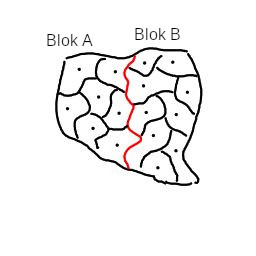
\includegraphics{5050.jpg}
\end{center}

W bloku A znajdowały się dwie partie: PZK (Partia Zwolenników Kawy) i PZH (Partia Zwolenników Herbaty), z których każda otrzymała po 25\% głosów w ogólnokrajowym głosowaniu. W bloku B znajdowała się partia PZA (Partia Zwolenników Alkoholu) oraz inne partie, które nie przekroczyły progu 5\%. Przedstawmy liczbę uzyskanych głosów w PZA:

\begin{tabular}{|c|c|}\hline
	Nazwa       & Głosy\\\hline
	Żubr        & \textbf{19995}\\\hline
	Żubrówka    & \textbf{2}\\\hline
	Soplica     & \textbf{2}\\\hline
	Pan Tadeusz & \textbf{1}\\\hline
\end{tabular}\\

\Komentarz{I tym oto sposobem wygrywają osoby, które dostają 2 lub 1 głos.}

\subsection{\href{http://www.racjonalista.pl/kk.php/s,9848/k,3}{Prawo Ciesielskiego}}

Rozważmy głosowanie względem 2 partii z 7 mandatami:

\begin{tabular}{|c|c|c|c|c|c|c|}\hline
	Nazwa        & Głosy:1 & :3 & :5  & :7  & :9  & Mandaty\\\hline
	Kelnerzy     & \textbf{1050} & \textbf{350} & \textbf{210} & 150 & 117  & 4\\\hline
	Sportowcy    & \textbf{1008} & \textbf{336} & 202  & 144 &      & 3\\\hline
\end{tabular}\\

Partia \textbf{Sportowcy} postanowiła się rozdzielić na dwie partie i startować osobno:

\begin{tabular}{|c|c|c|c|c|c|c|}\hline
	Nazwa        & Głosy:1 & :3 & :5  & :7  & :9  & Mandaty\\\hline
	Kelnerzy     & \textbf{1050} & \textbf{350} & \textbf{210} & 150 & 117  & 3\\\hline
	Piłkarze     & \textbf{504}  & \textbf{168} & 101  &     &      & 2\\\hline
	Siatkarze    & \textbf{504}  & \textbf{168} & 101  &     &      & 2\\\hline
\end{tabular}\\

\Komentarz{Tym oto sposobem partia \textbf{Sportowcy} zdobyła większość.}

	
\newpage

\section{Treść właściwa}
\subsection{Metody głosowania (system wyborczy)}

Wprowadźmy kilka oznaczeń, niech: \\
\\ $W$ - zbiór wszystkich wyborców, \\
$K$ - zbiór wszystkich kandydatów.
\begin{itemize}
	\item Ten sam układ głosów (zestaw głosów) daje ten sam wynik (funkcja).
	\item Każdy układ głosów daje jakiś wynik (może być $\emptyset$).
\end{itemize}

\begin{definition}[Model]
	Model to układ głosów (z przyporządkowanymi wyborcami).
\end{definition}

\begin{definition}[Metoda anonimowa]
	Metoda jest anonimowa, \textit{wtedy i tylko wtedy} (w skrócie: \witw), gdy wszyscy wyborcy są traktowani tak samo, \witw $\forall_{x,y \in W}$ zamiana głosów $x$ i $y$ nie zmienia wyniku.
\end{definition}

\Komentarz{Alternatywnie, metoda nie jest anonimowa \witw $\exists_{x,y \in W}$ takie, że zamiana głosów $x$ i $y$ \textit{istotnie} zmienia wynik.}

\begin{definition}[Metoda neutralna]
	Metoda jest neutralna, \witw wszyscy kandydaci są traktowani tak samo, \witw $\forall_{x,y \in K}$ zamiana ról $x$ i $y$ nie zmienia wyniku.
\end{definition}

\Komentarz{Alternatywnie, metoda nie jest neutralna \witw $\exists_{x,y \in K}$ takie, że zamiana ról $x$ i $y$ \textit{istotnie} zmienia wynik, dokładniej definiując:\\
jeśli $\exists{k_1,k_2\in K}: W_1=\{w_{1},w_{2},\dots,w_{i}\}$ głosowali na $k_1$, a $W_2=\{w_{i+1},w_{i+2},\dots,w_{j}\}$ głosowali na $k_2$ to jeżeli kandydaci Ci "zamienią się" wyborcami (zbiorami $W_1,W_2$), to $k_1$ i $k_2$ zamienią się wynikami.}

\begin{definition}
	Trzy rodzaje metod ze względu na wyniki:
\end{definition}

\begin{enumerate}[1)]
	\item Metoda zwycięzcy (MZ) – wybiera zwycięzcę (zwycięzców),
	\item Metoda porządkowa (MP) – wynik to słaby porządek na zbiorze $K$,
	\item Metoda rozdziału (MR) – wynik to podział pewnych dóbr między kandydatów.
\end{enumerate}
\subsubsection{Metoda zwyciężcy}
\begin{definition}[Klasyczna metoda zwycięzcy]
	Klasyczna metoda zwycięzcy (klasyczna MZ) polega na tym, że każdy wyborca głosuje na dokładnie jednego kandydata. Zbiór
	$$\Sigma = \{m:W\rightarrow K\}$$
	jest zbiorem modeli, gdzie $m$ jest modelem. Klasyczną metodę zwycięzcy możemy opisać funkcją
	$$f: \Sigma \rightarrow P(K).$$
\end{definition}

\begin{definition}[Semi-klasyczna metoda zwycięzcy]
	Semi-klasyczna MZ polega na tym, że każdy wyborca głosuje na co najmniej jednego kandydata:
	$$\Sigma = \{m:W\rightarrow P(K)\setminus \emptyset\}.$$
	Metodę tę można opisać funkcją
	$$f: \Sigma \rightarrow P(K).$$
\end{definition}

\begin{definition}[Metoda efektywna]
	Metoda zwycięzcy jest efektywna \witw zawsze wyłania przynajmniej jednego zwycięzcę.
\end{definition}

\begin{example}[Przykłady metod głosowania]
	\textbf{Metody klasyczne:}
\end{example}
\begin{enumerate}[1)]
	\item Dyktatura – $\exists_{\;p \in W}$: wynik jest tożsamy z głosem $p$.
	\item Monarchia – dany kandydat $k \in K$ wygrywa niezależnie od głosowania.
	\item Metoda większości – wygrywa kandydat (lub kandydaci), który(a) otrzymał(a) najwięcej głosów.
	\item Metoda bezwzględnej większości – wygrywa kandydat $k \in K$, który otrzymał co najmniej $\lfloor\frac{\# W}{2}\rfloor + 1$ głosów.
	\item Metoda super większości – wygrywa kandydat, który uzyskał co najmniej $q$ głosów, gdzie $q > \frac{\# W}{2}$.
	\item Metoda status quo – \textit{Założenie:} $\exists$ pewien stan z jednym zwycięzcą.
	\\ Głosowanie metodą większości (lub super większości):
	\begin{itemize}
		\item jeśli metoda daje wynik, zwycięża "nowy" kandydat,
		\item jeśli metoda nie daje wyniku, zwycięża dotychczasowy kandydat.
	\end{itemize}
	Przykład: referendum.
	\item Metoda większości ważonej – $(W = \{a_1,\dots,a_n\})$, gdzie głos $a_i$ ma wagę $w_i \geq 0$. Wygrywa ten, kto otrzyma ponad $\frac{w_1 + \dots + w_n}{2}$ punktów.
	\item Metoda głosowania blokowego – $W = W_1 \cup \dots \cup W_n$, gdzie $W_k$ to zbiór wyborców bloku. $W_k$ podejmuje decyzję większością głosów. W przypadku remisu wybierają zwycięzcę w $W_k$. Głos z $W_k$ ma wagę $i_k$. Wygrywa kandydat z największą liczbą punktów.
	
	\textbf{Metody semi-klasyczne:}
	\item Metoda n-głosów – każdy wyborca głosuje na $n$ kandydatów, a zwycięża ten, kto uzyska najwięcej głosów.
	\item Szeroka metoda n-głosów - każdy głosuje na n kandydatów, ale mamy n zwyciężców (lub więcej w przypadku remisu na ostatnim "wygrywającym" miejscu)
	
	\textbf{Metoda ani klasyczna, ani semi-klasyczna:}
	\item Metoda punktowa – każdy wyborca $w \in W$ ma do rozdysponowania $p$ punktów $(p \in \mathbb{N})$ między kandydatów. Zwycięża kandydat z największą liczbą punktów.
\end{enumerate}

\begin{definition}[Metoda decyzyjna]
	Metoda zwycięzcy jest decyzyjna \witw w każdym modelu wyłania dokładnie jednego zwycięzcę.
\end{definition}

\begin{definition}[Metoda prawie decyzyjna]
	Metoda zwycięzcy jest prawie decyzyjna \witw w każdym modelu wyłania co najwyżej jednego zwycięzcę. Sytuacja, w której nie ma zwycięzcy, zachodzi wtedy, gdy więcej niż jeden kandydat uzyskał tę samą, najwyższą liczbę punktów.
\end{definition}

\begin{exercise}[Z ćwiczeń]
	Zbadaj kto jest zwycięzcą w głosowaniu przez 99 osób na kandydatów: \textbf{Anastazy}, \textbf{Bermudy}, \textbf{Cezary}, jeśli otrzymano następujące wyniki metodą porządkową:
\end{exercise}

	\begin{tabular}{|c|c|}\hline
		Liczba głosów	& Wynik porządkowy\\\hline
		18        		& ABC\\\hline
		15    			& ACB\\\hline
		24     			& BAC\\\hline
		8 				& BCA\\\hline
		16     			& CAB\\\hline
		18 				& CBA\\\hline
	\end{tabular}\\
	
\begin{exercise}
	Dane są wyniki głosowania:\\\\
	\begin{tabular}{|c|c|}\hline
		Imię		& Liczba głosów\\\hline
		Jaś        	& 100\\\hline
		Małgosia    & 1\\\hline
	\end{tabular}\\\\
	Zrób tak, by Małgosia wygrała.
\end{exercise}

\begin{exercise}
	Uzupełnij tabelę:\\
	\begin{tabular}{|c|c|c|c|}\hline
		& Anonimowa & Neutralna & Efektywna\\\hline
		Dyktatura   &-&+&+\\\hline
		Monarchia   &+&-&+\\\hline
		Metoda Większości &+&+&+\\\hline
	\end{tabular}\\
\end{exercise}




	\begin{definition}[Kryterium jednoznacznej bezwzględnej większości]
		Metoda zwycięzcy (MZ) spełnia kryterium jednoznacznej bezwzględnej większości, \textit{wtedy i tylko wtedy}, gdy kandydat, który otrzyma ponad 50\% głosów, jest jedynym zwycięzcą.
	\end{definition}
	
	\begin{stwierdzenie}
		Mamy klasyczną metodę zwycięzcy, taką że $\# K=2$, a głosowanie odbywa się według zasady bezwzględnej większości. Wówczas metoda jest prawie decyzyjna.
	\end{stwierdzenie}
	
	\textit{Dowód:}
	\begin{enumerate}[1$^\circ$]
		\item Załóżmy, że liczba wyborców $\# W$ jest nieparzysta - OK.
		\item Liczba wyborców $\# W$ jest parzysta:
		\begin{itemize}
			\item jeden kandydat ma więcej niż 50\% głosów - OK.
			\item remis, czyli obaj mają po 50\% - nie ma zwycięzcy (dlatego metoda jest prawie decyzyjna).
		\end{itemize}
		\begin{flushright}$\square$\end{flushright}
	\end{enumerate} 
	
	\begin{stwierdzenie}
		Metoda jest decyzyjna $\Rightarrow$ metoda jest prawie decyzyjna.
	\end{stwierdzenie}
	
	\begin{definition}[Metoda monotoniczna ze względu na zwycięzcę]
		\textbf{Z:} MZ - klasyczna lub semi-klasyczna.
		Metoda jest monotoniczna ze względu na zwycięzcę, \textit{wtedy i tylko wtedy}, gdy kandydat $A$ jest zwycięzcą, a jeśli wybierzemy kandydata $B$ różnego od $A$ ($B\neq A$) oraz jego grupę wyborców, to jeśli ta grupa zmieni swoje głosy bez straty dla $A$ (czyli zmiana nastąpi zgodnie z następującymi dozwolonymi operacjami):
		
		\begin{tabular}{|c|c|c|}
			\hline
			M & $\Rightarrow$ & N \\\hline
			A B & $\Rightarrow$ & A B \\\hline
			- - & $\Rightarrow$ & - - \\\hline
			+ + & $\Rightarrow$ & + + \\\hline
			- + & $\Rightarrow$ & + - \\\hline
		\end{tabular}
		
		to: $\Rightarrow$ $A$ nadal wygrywa.
	\end{definition}
	
	\Komentarz{Czyli, jeżeli ktoś, kto nie głosował na zwycięzcę ($A$), a głosował na kandydata $B$, zmieni swój głos na zwycięzcę ($A$), to ($A$) nadal wygrywa.}
	
	\begin{definition}[Metoda kwoty]
		MZ klasyczna lub semi-klasyczna jest metodą kwoty (większości kwalifikowanej), \textit{wtedy i tylko wtedy}, gdy istnieje $q$ (kwota), taka że liczba głosów o tej własności, że kandydat $A$ jest zwycięzcą \textit{wtedy i tylko wtedy}, gdy $A$ otrzymał co najmniej $q$ głosów.
		
		\Komentarz{Często kwota wyrażana jest w procentach, a wówczas stosuje się nieraz nierówność słabą.}
	\end{definition}
	\begin{theorem}[Maya - \textit{Kenneth Maya, 1952r}]
		\textbf{Z:} Klasyczna metoda zwycięzcy oraz $\# K = 2$. Jeżeli metoda ta jest metodą:
		\begin{enumerate}[(1)]
			\item anonimową
			\item neutralną
			\item monotoniczną ze względu na zwycięzcę
			\item prawie decyzyjną
		\end{enumerate}
		$\Rightarrow$ jest metodą bezwzględnej większości.
	\end{theorem}
	
	\textit{Dowód:}
	Załóżmy, że $A,B$ to kandydaci.\\
	$\overset{(1)}{\Rightarrow}$ interesują nas liczby głosów, które otrzymali kandydaci. Załóżmy:\\
	$A$ - $a$ głosów\\
	$B$ - $b$ głosów\\
	Rozpatrzmy zatem przypadki:\\
	\begin{enumerate}[1$^\circ$]
		\item $\# W = 2n$ (parzysta), rozważmy dwa podprzypadki:
		\begin{enumerate}[a)]
			\item Jeśli $a=n$, $b=n$.\\
			\textbf{Hipoteza:} $A$ wygrywa (analogicznie, jeżeli nie wygrywa $B$), a metoda jest neutralna, to przy wymianie wyborców $\overset{(2)}{\Rightarrow}$ $B$ wygrywa (nie wygrywa $A$) $\Rightarrow$ $A$ i $B$ wygrywają jednocześnie (nie wygrywa żaden) $\Rightarrow$ co prowadzi do \faBolt (bo żaden z nich nie ma ponad 50\%).
			
			\item Jeśli $a>b$.\\
			\textbf{Hipoteza:} $B$ wygrywa, wtedy $a-b$ wyborców zmienia głosy z $A$ na $B$, $\overset{(3)}{\Rightarrow}$ $B$ dalej wygrywa. Teraz $B$ ma $a$ głosów, $\overset{(2)}{\Rightarrow}$ $A$ wygrywa, $\overset{(4)}{\Rightarrow}$ $A$ wygrywa i ma ponad połowę głosów.
		\end{enumerate}
		
		\item Niech $\# W = 2n+1$ (nieparzysta).\\
		Niech $a>b$.\\
		\textbf{Hipoteza:} $B$ wygrywa, $a-b$ wyborców zmienia głosy i, jak w 1a), udowadniamy, że $B$ musi mieć ponad połowę głosów.
	\end{enumerate}
	
	Tak więc zawsze wygrywa ten, kto ma ponad połowę głosów.
	\begin{flushright}$\square$\end{flushright}
	\subsubsection{MZU - Metoda zakładająca uporządkowanie}
	\begin{definition}[Metoda zakładająca uporządkowanie]
		Metoda zwycięzcy jest metodą zakładającą uporządkowanie (MZU) \textit{wtedy i tylko wtedy}, gdy $\forall_{w\in W}$ ustala $K$ kandydatów w liniowym porządku, a jego głos zależy od tego porządku.
	\end{definition}
	
	\textbf{Zapis:}\\\\
	$A\overset{w,m}{<}B$ w modelu $m$ oznacza, że wyborca $w$ stawia $B$ wyżej niż $A$.\\
	$A\overset{w}{<}B$ - gdy wiadomo, jaki model.
	
	\begin{example}
		\begin{enumerate}[1.]
			\item Metoda punktów Bordy (Jean Charles de Borda, 1733–1799, inżynier wojskowy) – Każdy wyborca przydziela punkty od $n-1$ do 0:\\
			1 miejsce - $n-1$ punktów\\
			2 miejsce - $n-2$ punktów\\
			$\vdots$ \\
			$n-1$ miejsce - 1 punkt\\
			$n$ miejsce - 0 punktów\\\\
			Zwycięża ten, kto otrzyma największą liczbę punktów.
			
			\item Metoda Hare'a (Sir Thomas Hare, 1806–1891, Anglia, prawnik, 1857 r.) – Polega na odrzucaniu tego kandydata (tych kandydatów), który ma najmniej pierwszych miejsc, i głosowaniu dalej (listy pozostają z usunięciem odrzuconego kandydata), aż ktoś uzyska ponad $50\%$ głosów. Gdy następuje remis i nie ma kogo odrzucić, wszyscy wygrywają.
			
			\item Metoda Coombsa (Clyde Coombs, 1912–1988, USA, psycholog) – Wypisujemy kolejność wyników głosowania, odrzucamy kandydata (lub kandydatów jeżeli ktoś zostanie), który ma najwięcej ostatnich miejsc, i głosujemy dalej, aż ktoś uzyska ponad $50\%$ pierwszych miejsc. Gdy nie można nikogo odrzucić, wygrywają wszyscy, którzy pozostali.
			
			\item Metoda odrzuceń ostatniego – Jak w metodzie Coombsa, przy czym odrzucamy „do oporu”. Gdy nie można nikogo więcej odrzucić, wygrywają wszyscy, którzy pozostali.
			
			\begin{example}
				Różnica między metodą Coombsa a metodą odrzucania ostatniego.\\
				
				\textbf{Metoda Coombsa}\\
				\begin{tabular}{|c|c|c|c|}\hline
					Liczba: & 4 & 2 & 3 \\\hline
					I pozycja & C & \textbf{B} & \textbf{B} \\\hline
					II pozycja & A & C & A \\\hline
					III pozycja & B & A & C \\\hline
				\end{tabular}\\\\
				Wygrywa $B$, bo ma ponad 50\% pierwszych miejsc.\\\\
				
				\textbf{Metoda odrzuceń ostatniego}\\
				\begin{tabular}{|c|c|c|c|}\hline
					Liczba: & 4 & 2 & 3 \\\hline
					I pozycja & C & B & B \\\hline
					II pozycja & \xout{A} & C & A \\\hline
					III pozycja & \sout{B} & \xout{A} & C \\\hline
				\end{tabular}\\\\
				Kolejność odrzuceń: B, A, C – C wygrywa.
			\end{example}
			
			\item Metoda Copelanda (Arthur H. Copeland, 1898–1970, matematyk) – Porównujemy parami kandydatów. Ten, kto więcej razy zostaje oceniony wyżej, dostaje 1 pkt, a w przypadku remisu obaj dostają po 0,5 pkt.
			
			$\#\{m:A\overset{m}{<}B\}$\\
			$\#\{m:B\overset{m}{<}A\}$\\
			
			Decyduje suma punktów (zwycięzców może być więcej niż jeden).
			
			\item Metoda turniejowa (Z: $\# W = 2n+1$ nieparzysta) – $k_1$ porównujemy z $k_2$ (metodą powyżej),a następnie zwycięzcę pierwszego porównania porównujemy z $k_3$ itd.
			
			\item Metoda pozycyjna – Wyborcy przyznają punkty kandydatą w postaci $P(p_1, p_2, \dots, p_n)$, gdzie $p_1\geq p_2 \geq \dots \geq p_n$. np.\\ 
			1 miejsce – $p_1$ punktów \\
			2 miejsce – $p_2$ punktów\\ itd.\\\\
			Zwycięża ten z największą liczbą punktów.\\
			
		\end{enumerate}
			
			
		\textbf{UWAGA – w szczególności:}\\
		Metoda Bordy: $P(n-1, n-2, \dots, 1, 0)$\\
		Metoda większości: $P(1,0, \dots, 0)$\\
		Metoda $k$ głosów: $P(\underset{\text{k razy}}{1,1,\dots,1}, 0, \dots, 0)$
	\end{example}
		
		\begin{definition}[Monotoniczność ze względu na transpozycję]
			MZU jest monotoniczna ze względu na transpozycje \witw $\forall_{M-\text{model}} \forall_{w\in W} \forall_{A,B\in K}$, jeśli w $M$ głosuje się $[\Delta, B, A, *]$ i w $M$ wygrywa $A$, to w $N$, gdzie zmiana polega na $[\Delta, A, B, *]$, również wygrywa $A$.
		\end{definition}
		
		\Komentarz{Zmiana polega na zamienieniu kolejności uporządkowania $A$ i $B$. Dodatkowo porządek ten był na wykładzie zapisany pionowo. $\begin{bmatrix}
				\Delta\\
				A\\
				B\\
				*
			\end{bmatrix}$
		}
		
		{\textbf{Umowa:}} Jeśli nie jest zaznaczone inaczej, to w $K,W$ różne oznaczenia oznaczają różnych kandydatów (wyborców).
		
		\begin{definition}[Słaba zasada Pareto]
			MZU spełnia słabą zasadę Pareto \witw $\forall_M (\exists_{A,B\in K}\forall_{w\in W} A\overset{w,M}{<}B) \Rightarrow A$ nie wygrywa w $M$.
		\end{definition}
		
		\begin{definition}[Kandydat Condorceta]
			$A\in K$ jest kandydatem Condorceta (zwycięzcą Condorceta) \witw w "bezpośrednich porównaniach" $A$ jest lepszy od każdego innego kandydata \witw $\forall_{B \in K}: B\neq A \quad \#\{w: B\overset{w,M}{<}A\}>\#\{w: B\overset{w,M}{>}A\}$.
		\end{definition}
		
		\begin{definition}[Przegrany Condorceta]
			$A\in K$ to przegrany Condorceta (w modelu $M$) \witw $\forall_{B \in K}: B\neq A \quad\#\{w: B\overset{w,M}{<}A\}<\#\{w: B\overset{w,M}{>}A\}$.
		\end{definition}
		
		\begin{definition}[Kryterium Condorceta]
			Metoda spełnia kryterium Condorceta \witw $\forall_M:$ Istnieje kandydat Condorceta (w $M$) $\Rightarrow A$ - jedyny zwycięzca w $M$.
		\end{definition}
		
		\begin{definition}[Kryterium przegranych Condorceta]			
			Metoda spełnia kryterium przegranych Condorceta \witw $\forall_M:$ Istnieje przegrany Condorceta $A$ w $M$ $\Rightarrow A$ nie wygrywa w $M$.
		\end{definition}
		
		\begin{definition}[Metoda jednoznacznie większościowa]
			Metoda jest jednoznacznie większościowa \witw $\forall_M$ kandydat $A$ w $M$ ma ponad połowę pierwszych miejsc $\Rightarrow A$ - jedyny zwycięzca.
		\end{definition}
		
		\begin{definition}[Metoda słabo niezależna od ubocznych opcji]
			Metoda słabo niezależna od ubocznych opcji spełnia warunek niezależności porażki od ubocznych opcji (spełnia słaby warunek $IIA$) \witw
			
			$\forall_{A,B\in K} \forall_{M,N - modele}$ spełnia 
			$\begin{bmatrix}
				\forall_{w\in W} (B\overset{w,M}{<}A) \text{\witw} (B\overset{w,N}{<}A) \\
				\text{A wygrywa w M, B nie wygrywa w M}		 
			\end{bmatrix}$	$\Rightarrow$ B nie wygrywa w N.\\\\
			
			Innymi słowy: zmiany nie wpływające na relacje przegrany-zwycięzca nie mogą dać przegrywającemu zwycięstwa.		
			
		\end{definition}
		
		\begin{theorem}
			MZU, anonimowa, neutralna $\Rightarrow$ metoda nie jest decyzyjna.
		\end{theorem}
		\textit{Dowód.} Rozważmy $\# K = 2$, $\# W = 2n$ i otrzymane głosy.\\
		
		\begin{tabular}{|c|c|c|}\hline
			Głosy&n&n\\\hline
			1&A&B\\\hline
			2&B&A\\\hline
		\end{tabular}\\\\
		\textbf{Hipoteza:} Metoda decyzyjna to np. wygrywa $A \Rightarrow$ wygrywa $B$ \faBolt\\
		Analogicznie zachodzi dla $A$.
		
		\begin{flushright}$\square$\end{flushright}
		
		\begin{example}[Paradoks Condorceta]
			Rozważmy następującą tabelę:\\
			\begin{tabular}{|c|c|c|c|}\hline
				Głosy&9&10&11\\\hline
				1&A&B&C\\\hline
				2&B&C&A\\\hline
				3&C&A&B\\\hline
			\end{tabular}\\
			
			Zachodzi $A>B$, $B>C$, $C>A$. Mamy więc grę w "kamień, papier, nożyce."
		\end{example}
		
		\begin{theorem}
			MZU spełnia kryterium Condorceta $\Rightarrow$ jest jednoznacznie większościowa.
		\end{theorem}
		\textit{Dowód.} A ma ponad połowę pierwszych miejsc $\Rightarrow$ A - kandydat Condorceta $\Rightarrow$ A jest jedynym zwycięzcą.		
		
		\begin{flushright}$\square$\end{flushright}
		
		\begin{theorem}
			MZU spełnia słabe $IIA$, a $A$ spełnia kryterium Condorceta $\Rightarrow$ spełnia słabą zasadę Pareto.
		\end{theorem}
		\textit{Dowód.} Rozważmy $M$ $\forall_{W} A\overset{w,M}{<}B \overset{?}{\Rightarrow}$ $A$ nie wygrywa w $M$.
		
		Rozważmy model $N$: dla każdego wyborcy przesuwamy $A$ i $B$ na szczyt, $[B,A,reszta]$ $A\overset{w,M}{<}B$ \witw $A\overset{w,N}{<}B$.
		
		W $N$: $B$ jest kandydatem Condorceta.
		
		W $N$: $B$ jest jedynym zwycięzcą, $B$ wygrywa, $A$ nie wygrywa. 
		
		$\overset{\textbf{Słabe IIA}}{\Rightarrow}$ $A$ nie wygrywa w $M$.
		\begin{flushright}$\square$\end{flushright}
		
		\begin{theorem}
			MZU, monotoniczna ze względu na transpozycje, \witw $\forall_{M - \text{model}} \forall_{A\in K} \forall_{B_1,\dots,B_n\in A} (A\neq B, \text{ ale może być } B_i=B_j)$
			$\forall_{w_1,\dots,w_n\in W}$ (może być $w_i=w_j$)
			
			Jeżeli w modelu $M$ wygrywa $A$, to model $N$ utworzony przez $[\Delta, B_i, A, *] \rightarrow [\Delta, A, B_i, *]$ dla $i=1,\dots,n$ $\Rightarrow$ w $N$ dalej wygrywa $A$.
			
		\end{theorem}
		
		\textit{Dowód.} $\Leftarrow$ oczywiste.
		
		$\Rightarrow$ Stosujemy założenie $n$ razy (robimy $n$ skoków i dalej wygrywa $A$).
		
		\begin{example}
			
		\end{example}
		
		\begin{enumerate}[1.]
			\item Metoda Blacka (1908-1991, ekonomista) - jeśli istnieje kandydat Condorceta, to on wygrywa. Jeśli nie istnieje, stosujemy punkty Bordy.
			\item Metoda Condorceta - jeśli istnieje kandydat, który w "bezpośrednim porównaniu" wygrywa lub remisuje z każdym innym \witw$\:$  on jest zwycięzcą.
			\item Metoda nominacji - każdy, kto ma co najmniej jedno pierwsze miejsce, wygrywa.
			\item Metoda ostatnich miejsc - każdy, kto nie ma żadnego ostatniego miejsca, wygrywa.
			\item Metoda prezydencka - rozważamy dwóch kandydatów z największą liczbą pierwszych miejsc. Porównujemy ich "bezpośrednio". Jeśli na drugim miejscu jest remis, wszyscy z drugiego miejsca "przechodzą do finału" i tam stosujemy metodę Copelanda.
		\end{enumerate}
		
		Metoda punktów Bordy jest monotoniczna ze względu na transpozycję.
		
		$A$ wygrywa. Niech $A$ zdobędzie 1 punkt więcej. Innym się nie zwiększyło $\Rightarrow$ $A$ dalej wygrywa.\\\\
		
		\begin{tabular}{|p{2.5cm}|p{2cm}|p{2cm}|p{2cm}|p{2cm}|c|p{2cm}|}\hline
			Metoda & Kryterium Condorceta & Kryterium przegranego Condorceta & Słaba zasada Pareto & Monoto- niczność ze względu na transpozycję & IIA & Jedno- znaczna większość\\\hline
			Punkty Bordy   &-(1)&+&+&+&-(2)&-(1)\\\hline
			Hare'a   &-(3)&-(3)&+&-(4)&-(5)&+(O)\\\hline
			Coombsa &-(14)&-(15)&+&-(13)&-(13)&+(O)\\\hline
			Odrzuceń ostatniego &-(11,12)&-(12)&+&-(13)&-(13)&-(11,12)\\\hline
			Copelanda &+&+&+&+&-(10)&+(O)\\\hline
			Większości &-(3)&-(3)&+(O)&+&-(6)&+\\\hline
			Dyktatura &-(7)&-(7)&+&+(O)&+&-(7)\\\hline
			Terminażowa &+&+&-(8)&+&-(9)&+\\\hline
		\end{tabular}\\\\
		
		\begin{enumerate}[D1)]
			\item \textbf{Metoda Bordy, Kryterium przegranego Condorceta} $\forall_w A<B$ Punkty $A$ < Punkty $B$. W punktacji $A$ zdobywa 1 punkt za każdą parę $(B, w)$, w której wyborca $w$ umieszcza $B$ wyżej niż $A$. 
			
			$A$ jest przegranym Condorceta. Mamy $k$ kandydatów, $n$ wyborców, a kandydat $K_1,...,K_{n-1}$ otrzyma mniej niż $\frac{n}{2}$ punktów. W sumie, $A$ zdobywa mniej niż $\frac{k(k-1)}{2}$ punktów.
			
			Łączna pula punktów do rozdziału wynosi $n\cdot\frac{k(k-1)}{2}$ (suma ciągu arytmetycznego). Wszyscy razem zdobywają mniej niż $\frac{n(k-1)}{2}$ punktów, czyli łącznie mniej niż $\frac{k\cdot n \cdot (k-1)}{2}$.
			
			\item \textbf{Metoda Comba i Hare'a} Jeśli $\forall_w A \overset{w}{<} B$, to $A$ wcześniej odpadnie od $B$.
			
			\item \textbf{IIA dyktatura} Jeśli $A$ wygrywa, $B \overset{d,M}{<} A$, to $B$ nie może wygrać.
			
			\item \textbf{Metoda terminarzowa - Kryterium Condorceta} Kandydat Condorceta wygrywa z każdym i nie odda zwycięstwa.
			
			\item \textbf{Terminażowa - monotoniczność} Przy przesunięciu $A$ również wygrywa.
			
			\item \textbf{Metoda Copelanda} Gdy $A$ wygrywa z każdym, to zdobywa maksymalną liczbę punktów. Zasada Pareto: $\forall_w B \overset{w}{<} A \overset{?}{\Rightarrow} B$ nie wygrywa.
			
			Jeśli $B$ wygrywa w pojedynku z $C$, to również $A$ wygrywa z $C$. Wówczas punkty $A >$ punkty $B$, ponieważ $A$ zdobywa punkty za parę $(A, B)$, a zatem punkty $A$ są silniejsze.
			
			\item \textbf{Metoda Coombsa - Słaba zasada Pareto} Jeśli $\forall_w B \overset{w}{<} A$, to $A$ nie odpadnie, zanim $B$ nie odpadnie (czyli $B$ odpadnie wcześniej niż $A$).
		\end{enumerate}
		
		\begin{enumerate}[K1)]
			\item \begin{tabular}{|c|c|c|}\hline
				3os & 2os & Pkt\\\hline
				A & B & 2\\\hline
				B & C & 1\\\hline
				C & A & 0\\\hline
			\end{tabular}
			$A$ jest kandydatem Condorceta, natomiast otrzymano punkty: $\begin{bmatrix}
				A=6\ \text{pkt}\\
				B=7\ \text{pkt}\\
				C=2\ \text{pkt}\\
			\end{bmatrix}$
			
			\item \begin{tabular}{|c|c|c|c|}\hline
				1os & 2os & 2os & Pkt\\\hline
				C & A & B & 2\\\hline
				A & B & A & 1\\\hline
				B & C & C & 0\\\hline
			\end{tabular} $\Rightarrow$ \begin{tabular}{|c|c|c|c|}\hline
				1os & 2os & 2os & Pkt\\\hline
				C & A & B & 2\\\hline
				A & B & \textbf{C$\uparrow$} & 1\\\hline
				B & C & A & 0\\\hline
			\end{tabular}, wykorzystując transpozycję otrzymujemy wyniki $\begin{bmatrix}
				A=5 && A=7\\
				B=6 & \Rightarrow & B=6\\
				C=4 && C=2\\
			\end{bmatrix}$, czyli $A$ wygrywa.
			
			\item \begin{tabular}{|c|c|c|}\hline
				2os & 3os & 2os\\\hline
				A & B & C\\\hline
				C & A & A\\\hline
				B & C & B\\\hline
			\end{tabular} $\begin{bmatrix}
				A - \text{kandydat Condorceta}\\
				B - \text{przegrany Condorceta}\\
			\end{bmatrix}$, bo $A:B$ $4:3$ $\Rightarrow$ $A:C$ $5:2$, ale wygrywa $B$.
			
			\item \begin{tabular}{|c|c|c|c|}\hline
				6os & 5os & 4os & 2os\\\hline
				A & C & B & B\\\hline
				B & A & C & A\\\hline
				C & B & A & C\\\hline
			\end{tabular} $\Rightarrow$ \begin{tabular}{|c|c|c|c|}\hline
				6os & 5os & 4os & 2os\\\hline
				A & C & B & \textbf{A$\uparrow$}\\\hline
				B & A & C & B\\\hline
				C & B & A & C\\\hline
			\end{tabular}, wygrywał $B$, po zmianie $C$.
			
			\item \begin{tabular}{|c|c|c|}\hline
				2os & 1os & 2os\\\hline
				B & A & A\\\hline
				A & B & C\\\hline
				C & C & B\\\hline
			\end{tabular} $B$ nie wygrywa, $A$ wygrywa $\Rightarrow$\begin{tabular}{|c|c|c|}\hline
				2os & 1os & 2os\\\hline
				B & A & \textbf{C$\uparrow$}\\\hline
				A & B & A\\\hline
				C & C & B\\\hline
			\end{tabular}, wygrywa $B$
			
			\item \begin{tabular}{|c|c|c|}\hline
				2os & 3os & 2os\\\hline
				A & B & A\\\hline
				B & A & C\\\hline
				C & C & B\\\hline
			\end{tabular}, $A$ wygrywa, $B$ nie wygrywa $\Rightarrow$ \begin{tabular}{|c|c|c|}\hline
				2os & 3os & 2os\\\hline
				A & B & \textbf{C$\uparrow$}\\\hline
				B & A & A\\\hline
				C & C & B\\\hline
			\end{tabular}
			
			\item \begin{tabular}{|c|c|}\hline
				2os & 1os (\text{w tym jeden dyktator})\\\hline
				A & B\\\hline
				B & A\\\hline
			\end{tabular} $\begin{bmatrix}
				A \text{ - kandydat Condorceta}\\
				B \text{ - przegrany Condorceta}
			\end{bmatrix}$, wygrywa $B$.
			
			\item Ustawiamy kolejność: $ABCD$
			\begin{tabular}{|c|c|c|}\hline
				1os & 1os & 1os\\\hline
				A & C & B\\\hline
				B & A & D\\\hline
				D & B & C\\\hline
				C & D & A\\\hline
			\end{tabular} mamy $\begin{bmatrix}
				A > B\\
				A < C\\
				C > D\\
			\end{bmatrix}$, ostatecznie wygrywa $D$, mimo iż $D < B$.
			
			\item Ustawiamy kolejność $ABC$
			\begin{tabular}{|c|c|c|}\hline
				1os & 1os & 1os\\\hline
				C & B & A\\\hline
				A & C & B\\\hline
				B & A & C\\\hline
			\end{tabular} mamy $\begin{bmatrix}
				A > B\\
				A < C\\
			\end{bmatrix}$, wygrywa $C$ $\Rightarrow$ \begin{tabular}{|c|c|c|}\hline
				1os & 1os & 1os\\\hline
				C & B & B\\\hline
				A & C & \textbf{A$\uparrow$}\\\hline
				B & A & C\\\hline
			\end{tabular}, $B$ wygrywa.
			
			\item \begin{tabular}{|c|c|c|c|}\hline
				2os & 2os & 1os & 1os\\\hline
				A & C & D & B\\\hline
				D & A & B & C\\\hline
				B & B & C & D\\\hline
				C & D & A & A\\\hline
			\end{tabular} otrzymujemy kolejno wyniki: $\begin{bmatrix}
				\textbf{A} > B\:(4:2) & \textbf{B} > C\:(4:2)\\
				A < \textbf{C}\:(2:4) & \textbf{B = D}\:(3:3)\\
				\textbf{A} > D\:(4:2) & \textbf{C = D}\:(3:3)\\
			\end{bmatrix}$, przyznano punkty $\begin{bmatrix}
				A\text{ -2 pkt}\\
				B\text{ -1,5 pkt}\\
				C\text{ -1,5 pkt}\\
				D\text{ -1 pkt}\\
			\end{bmatrix}$, $A$ wygrywa, $C$ nie wygrywa.
			
			Po zmianie: \begin{tabular}{|c|c|c|c|}\hline
				2os & 2os & 1os & 1os\\\hline
				A & C & D & B\\\hline
				D & A & B & C\\\hline
				\textbf{$\uparrow$} & B & C & D\\\hline
				B & D & A & A\\\hline
			\end{tabular} oraz punktacje: $\begin{bmatrix}
				A\text{ -2 pkt}\\
				B\text{ -0,5 pkt}\\
				C\text{ -2,5 pkt}\\
				D\text{ -1 pkt}\\
			\end{bmatrix}$, $C$ wygrywa.
			
			\item \begin{tabular}{|c|c|c|}\hline
				4os & 2os & 3os\\\hline
				C & B & B\\\hline
				A & C & A\\\hline
				B & A & C\\\hline
			\end{tabular} $B$ ma najwięcej głosów pierwszych, czyli jest kandydatem Condorceta, ale kolejność odrzuceń to $B$, $A$, więc wygrywa $C$.
			
			\item \begin{tabular}{|c|c|c|}\hline
				2os & 1os & 2os\\\hline
				C & B & B\\\hline
				A & C & A\\\hline
				B & A & C\\\hline
			\end{tabular} $C$ to przegrany Condorceta, ale $C$ wygrywa.
			
			\item \begin{tabular}{|c|c|c|c|}\hline
				5os & 4os & 1os & 2os\\\hline
				A & B & C & B\\\hline
				C & A & B & C\\\hline
				B & C & A & A\\\hline
			\end{tabular}, $A$ wygrywa, $C$ i $B$ nie wygrywają.
			
			Przekształcamy do: \begin{tabular}{|c|c|c|c|}\hline
				5os & 4os & 1os & 2os\\\hline
				A & B & C & B\\\hline
				C & A & B & \textbf{A$\uparrow$}\\\hline
				B & C & A & C\\\hline
			\end{tabular}, $B$ wygrywa.
			
			\item \begin{tabular}{|c|c|c|c|c|}\hline
				2os & 1os & 1os & 1os & 2os\\\hline
				E & D & A & C & B\\\hline
				A & B & B & B & C\\\hline
				D & A & C & D & A\\\hline
				C & E & E & E & D\\\hline
				B & C & D & A & E\\\hline
			\end{tabular}
			$B$ -kandydat Condorceta, $B$ odpada w I turze
			
			\item \begin{tabular}{|c|c|c|c|}\hline
				2os & 2os & 2os & 1os\\\hline
				D & B & C & B\\\hline
				C & D & B & C\\\hline
				A & A & A & D\\\hline
				B & C & D & A\\\hline
			\end{tabular} $A$-przegrany Condorceta, ale $A$ wygrywa
			 
		\end{enumerate}
		
		\begin{lemma}[Lemat o decyzyjności]
			Z: MZU, efektywna, $\#K\geq3$, $\#W\geq2$.
			Metoda spełnia słabą zasadę Pareto i słabe IIA
			$\Rightarrow$ jest decyzyjna.
		\end{lemma} \newpage
		Dowód: Wiemy, że zwycięzca istnieje (chcemy wykazać, że jest jedyny).
		Załóżmy, że $A$ i $B$ są zwycięzcami w modelu $M$ oraz
		$W=X\cup Y$ \begin{tabular}{|c|c|}\hline
			X & Y \\\hline
			\vdots & \vdots \\\hline
			A & B \\\hline
			\vdots & \vdots \\\hline
			B & A \\\hline
			\vdots & \vdots \\\hline
		\end{tabular} 
		Niech $C$ - inny kandydat
		
		Tworzymy model
		$\underset{Q}{\begin{tabular}{|c|c|}\hline
			X & Y \\\hline
			A & C\\\hline
			C & B \\\hline
			B & A \\\hline
			\dots & \dots \\\hline
		\end{tabular}}$
		, w którym relacje $A/B$ nie są zmienione.
		
		Kto wygrywa w $Q$?
		Na pewno nie $B$, bo $\forall_w \; B\overset{w}{<}C$, ale również nie $A$ (z IIA).
		
		Jeżeli w $Q$ $A$ wygrywa, $B$ nie $\Rightarrow$ w $M$ $B$ nie wygrywa \faBolt 
		
		Zatem wygrywa $C$.
		
		Rozważmy model $R$ $\underset{R}{\begin{tabular}{|c|c|}\hline
			X & Y \\\hline
			A & B\\\hline
			B & C \\\hline
			C & A \\\hline
			\dots & \dots \\\hline
		\end{tabular}}$
	
		Kto wygrywa w $R$? - $A$, $B$ lub $C$ (Pareto)
		Ale nie wygrywa $C$ (z zasady Pareto). W $R$: relacje $A/C$ są takie same jak w $Q$.
		
		Załóżmy, że $A$ wygrywa w $R$ $\Rightarrow$ $C$ nie wygrywa w $Q$. Wobec tego w $R$ wygrywa $B$.
		
		Porównajmy $M$ i $R$: relacje $A$-$B$ w $M$ i $R$ są takie same. Wobec tego z IIA $\Rightarrow$ w $M$ $A$ nie wygrywa \faBolt
		\begin{flushright}$\square$\end{flushright}
		
		
		\begin{theorem}[Twierdzenie Arrowa dla metod zwycięzcy (1951)]
			Załóżmy: $\# K \geq 3, \#W\geq2$, MZU, efektywna, spełnia słabą zasadę Pareto i słabe IIA $\Rightarrow$ dyktatura.
		\end{theorem}
		
		D: Z lematu o decyzyjności $\Rightarrow$ jeśli zwycięzca istnieje, to jest jedyny.
		
		Czy istnieje jedyny zwycięzca? (pytanie) dyktatura.
		
		\begin{definition}[na potrzeby dowodu]
			$w\in W$ - dyktator $A$ z kontrolerem $B$ \witw \quad jeśli $A\overset{w}{<}B \Rightarrow$ $A$ nie wygrywa.
		\end{definition}
		
		Podzielimy dówód na 3 kroki:
		
		\begin{enumerate}[I krok - ]
			\item $\forall_{A,B \in K} \exists_{w\in W}$ dyktator nad $A$ z kontrolerem $B$.
			
			\item $w$-dyktator nad $A$ z kandydatem $B$ $\Rightarrow$ $w$ dyktator nad $B$ z kontrolerem $A$ (dyktatora nad parą $A$, $B$ oznaczamy $d(A,B)$).
			
			\item Jeżeli $w=d(A,B) \Rightarrow \forall_{D,E} w = d(D,E)$ (gdzie $D,E$ może być $A$ lub $B$).
		\end{enumerate}
		
		
		
		Wtedy ten $w$ z I kroku jest dyktatorem.
		\begin{tabular}{|c|}\hline
			$w$ \\\hline
			$A$ \\\hline
			$B_1$ \\\hline
			$B_2$ \\\hline
			\dots \\\hline
			$B_n$ \\\hline
		\end{tabular}
		
		\begin{enumerate}[Dow. I)]
			\item Niech $C$ będzie trzecim kandydatem. \begin{tabular}{|c|}\hline
				$C$ \\\hline
				$A$ \\\hline
				$B$ \\\hline
				wszyscy \\\hline
			\end{tabular}
			Wygrywa $C$. Jeden wyborca przesuwa $C$ do tyłu:
			\begin{tabular}{c|c}\hline
				inni & $W_1$ \\\hline
				$C$ & $A$ \\
				$A$ & $B$ \\
				$B$ & $C$ \\
				\vdots & \vdots \\
			\end{tabular}
			Wygrywa $C$ lub $A$.
			
			To samo z trzecim wyborcą:
			\begin{tabular}{c|c}\hline
				inni & $w_1$ $w_2$ \\\hline
				$C$ & $A$ \\
				$A$ & $B$ \\
				$B$ & $C$ \\
				\vdots & \vdots \\
			\end{tabular}
			Wygrywa $A$ lub $C$, i tak dalej, aż dojdzie do sytuacji:
			\begin{tabular}{|c|}\hline
				wszyscy \\\hline
				$A$ \\\hline
				$B$ \\\hline
				$C$ \\\hline
			\end{tabular}
			Wówczas wygrywa $A$ (z zasady Pareto), a $C$ nie.
			
			Pierwsze przejście, po którym $C$ nie wygrywa (musi takie zaistnieć). 
			
			$X, Y$ - grupy wyborców.
			
			$\underset{M_1}{\begin{tabular}{|c|c|c|}\hline
					X & w & Y \\\hline
					$C$ & $C$ & $A$ \\\hline
					$A$ & $A$ & $B$ \\\hline
					$B$ & $B$ & $C$ \\\hline
			\end{tabular}} \Rightarrow \underset{M_2}{\begin{tabular}{|c|c|c|}\hline
					X & w & Y \\\hline
					$C$ & $A$ & $A$ \\\hline
					$A$ & $B$ & $B$ \\\hline
					$B$ & $C$ & $C$ \\\hline
			\end{tabular}}$
			
			Pokażemy, że $w$ jest dyktatorem nad $B$ z kontrolerem $A$.
			
			Rozważmy $P$ - dowolny model, w którym $B\overset{w,P}{<}A$. 
			
			Niech $A/B$ oznacza pewną relację między $A$ i $B$.
			
			$\underset{P}{\begin{tabular}{|c|c|c|}\hline
				$W$ & $V$ & inni \\\hline
				$A/B$ & $A$ & $A/B$ \\\hline
				& $B$ & \\\hline
				\vdots & \vdots & \vdots \\\hline
			\end{tabular}}
			\Rightarrow
			\underset{Q}{\begin{tabular}{|c|c|c|}\hline
				$W$ & $V$ & inni \\\hline
				$C$ & $A$ & $A/B$ \\\hline
				$A/B$ & $B$ & $C$ \\\hline
				\vdots & $C$ & \vdots \\\hline
				\vdots & \vdots & \vdots \\\hline
			\end{tabular}}$
			
						Kto wygrywa w $Q$? - $A$, $B$ lub $C$. Jednak relacje $B/C$ w modelach $Q$ i $M_1$ są takie same $\Rightarrow$ w $Q$ $B$ nie wygrywa (IIA). Z kolei relacje $A/C$ w $Q$ i $M_2$ są takie same $\overset{IIA}{\Rightarrow}$ w $Q$ $C$ nie wygrywa.
			
			W $Q$ wygrywa $A$, $B$ nie wygyrwa.
			
			Relacje $A/B$ w $P$ i $Q$ są takie same. $\Rightarrow$ w $P$ $B$ nie wygrywa.
			\newpage
			\item $w$ jest dyktatorem nad $B$ z kontrolerem $A$, $v$ jest dyktatorem nad $A$ z kontrolerem $B$
			
			\begin{tabular}{|c|c|c|}\hline
				$W$ & $V$ & inni \\\hline
				$A$ & $B$ & \\\hline
				$B$ & $A$ & \\\hline
				\vdots & \vdots & \\\hline
			\end{tabular}
			
			Wygrywa $A$ lub $B$ (z zasady Pareto).
			$B$ nie wygrywa (bo $w$), $A$ nie wygrywa (bo $v$) \faBolt
			\item Niech $w = d(A,B)$.
			1. Zauważmy, że $\forall_{D,E} \exists d(D,E)$.
			2. $\forall_{D,E}$ $w = d(D,E)$.
			
			D 2.1. Załóżmy, że $C$, oraz że $v = d(B,C)$ i $v \neq w$. 	
			\begin{tabular}{|c|c|c|}\hline
				$W$ & $V$ & inni \\\hline
				$C$ & $B$ & $C$ \\\hline
				$A$ & $C$ & $B$ \\\hline
				$B$ & $A$ & $A$ \\\hline
				\vdots & \vdots & \vdots \\\hline
			\end{tabular}
			
			Wygrywa $B$ lub $C$ (z zasady Pareto). $B$ nie wygrywa (bo $w$), $C$ nie wygrywa (bo $v$) \faBolt
			
			D 2.2. Zamieniamy $A$ i $B$ rolami, $v = d(A,C)$, i w ten sam sposób pokazujemy, że $w = d(A,C)$.
			
			D 2.3. $\overset{z 2.1 \text{ i } 2.2}{C \neq A,B}$ oraz $w = d(A,B)$, $w = d(A,C)$. Jeśli $D \neq A,C$, to podobne rozumowanie jak w 2.1 i 2.2 dla $A,C,D$ pokazuje, że $w = d(A,C) \Rightarrow w = d(C,D)$.
			
			Dla $C,d \neq A,B$ OK.
			Jeden z $C,D$ musi być równy $A$ lub $B$ (z 2.1 i 2.2).
			
		\end{enumerate}
	
\begin{flushright}$\square$\end{flushright}
\begin{wniosek}[Twierdzenie Arrowa o niemożliwości]
	Załóżmy, że $\# K \geq 3$, $\# W \geq 2$. Wówczas: nie istnieje metoda zakładająca uporządkowanie (MZU) efektywna, która jednocześnie spełnia następujące warunki:
	\begin{enumerate}[-]
		\item anonimowa,
		\item słabą zasadę Pareto,
		\item słabe kryterium niezależności od opcji ubocznych (IIA).
	\end{enumerate}
\end{wniosek}

\begin{example}[Przypadki szczególne w twierdzeniu Arrowa]
	\begin{enumerate}[1.]
		\item $\# K = 2$, $\# W$ nieparzyste — metoda większości jest decyzyjna.
		\item $\# K = 3$, $\# W = 5$ — reguła „$\geq 3$ pierwsze miejsca” wyłania zwycięzcę.
	\end{enumerate}
\end{example}

\begin{theorem}[Twierdzenie Taylora o niemożliwości]
	Dla $\# K \geq 3$, $\# W \geq 3$:  
	nie istnieje MZU efektywna, która spełnia jednocześnie kryterium Condorceta oraz słabe kryterium niezależności od ubocznych opcji (IIA).
\end{theorem}

\noindent \textbf{Dowód:}  
Z założeń IIA i kryterium Condorceta wynika słaba zasada Pareto.  
Słaba zasada Pareto wraz z IIA prowadzi do dyktatury (zgodnie z twierdzeniem Arrowa).  
Jednak dla $\# W \geq 3$, dyktatura nie spełnia kryterium Condorceta.  
\begin{flushright}$\square$\end{flushright}

Przypadek $\# W = 4$ jest znacznie prostszy do rozważenia.

\subsubsection{Metoda TAK/NIE}
$$
\begin{bmatrix}
	\Sigma = \{ M: W \rightarrow K \} & \Sigma = \{ M: W \rightarrow \{ \text{TAK}, \text{NIE} \} \} \\
	f:\Sigma \rightarrow P(K) & f:\Sigma \rightarrow \{ \text{TAK}, \text{NIE} \}
\end{bmatrix}
$$

\begin{example}[Szczególny przypadek metody status quo]
	Przypadek z dwoma kandydatami.
\end{example}
\begin{definition}[Założenia metody TAK/NIE]
	 Założenia:´
	
	\begin{itemize}
		\item $\forall_{w \in W} \; w : \text{TAK} \Rightarrow \text{wynik: TAK}$,
		\item $\forall_{w \in W} \; w : \text{NIE} \Rightarrow \text{wynik: NIE}$.
	\end{itemize}
\end{definition}



\begin{definition}[Koalicja wygrywająca]
	Podzbiór $A \subset W$ jest koalicją wygrywającą wtedy i tylko wtedy, gdy:  
	$$\{x \in A : x \text{ głosuje TAK} \} \Rightarrow \text{wynik: TAK.}$$
\end{definition}

\begin{definition}[Monotoniczność metody TAK/NIE]
	Metoda TAK/NIE jest monotoniczna wtedy i tylko wtedy, gdy:  
	$$
	\begin{bmatrix}
		A \subset A_1 \\
		A \text{ jest koalicją wygrywającą}
	\end{bmatrix}
	\Rightarrow A_1 \text{ jest koalicją wygrywającą.}
	$$
\end{definition}

\begin{definition}[Wyborca decydujący]
	Załóżmy, że $A$ jest koalicją wygrywającą.  
	Wyborca $p \in A$ jest decydujący dla $A$ wtedy i tylko wtedy, gdy $A \setminus \{p\}$ nie jest koalicją wygrywającą.
\end{definition}

\begin{definition}[Wskaźnik Banzhafa]
	Załóżmy, że $W = \{a_1, \dots, a_n\}$.  
	Wskaźnik Banzhafa dla $a_i$ jest równy liczbie:
	$$B(a_i) = \# \{ A : a_i \in A \; \text{i $a_i$ jest decydujący dla $A$} \}.$$
\end{definition}

\begin{definition}[Indeks Banzhafa (Penrose’a–Banzhafa)]
	Indeks Banzhafa dla $a_i$ definiuje się jako:
	$$I_B(a_i) = \frac{B(a_i)}{B(a_1) + \dots + B(a_n)}.$$
\end{definition}

	\begin{example}
		Trzech wyborców:
		\begin{itemize}
			\item $w_1 = 50$,
			\item $w_2 = 45$,
			\item $w_3 = 1$.
		\end{itemize}
		
		Do podjęcia decyzji TAK potrzeba 51 głosów.  
		\Komentarz{Zapis tego warunku: $W(51; 50, 45, 1)$ — gdzie $W(\text{min}; \text{wagi wyborców})$.}
		\newpage
		
		**Metoda liczenia wskaźnika Banzhafa (dla metod monotonicznych)**:
		
		ALGORYTM:  
		\begin{tabular}{c|cccc}
			Koalicje wygrywające $\setminus$ Wyborcy & $w_1$ & $w_2$ & \dots & $w_n$ \\ \hline
			$k_1$ & + & + & \dots & - \\
			$k_2$ & - & + & \dots & - \\
			\vdots & \vdots & \vdots & & \vdots \\
			$k_j$ & + & - & \dots & - \\
		\end{tabular}
	
		Legenda:
		\begin{itemize}
			\item $+$ (wyborca należy do koalicji),
			\item $-$ (wyborca nie należy do koalicji).
		\end{itemize}
	
		\Komentarz{Policzymy teraz wskaźniki Banzhafa dla $W(51;50,45,1)$}
		
		**Koalicje wygrywające**:
		\begin{itemize}
			\item $\{w_1, w_2\}$,
			\item $\{w_1, w_3\}$,
			\item $\{w_1, w_2, w_3\}$.
		\end{itemize}
	
		
	
		
		
		Liczba znaków $+$ dla wyborcy $w_1$ minus liczba znaków $-$ to wskaźnik Banzhafa.
		
		**Przykład**:
		\begin{tabular}{c|ccc}
			Koalicja & $w_1$ & $w_2$ & $w_3$ \\ \hline
			$\{w_1, w_2\}$ & + & + & - \\
			$\{w_1, w_3\}$ & + & - & + \\
			$\{w_1, w_2, w_3\}$ & + & + & + \\
			& 3 =(3-0) & 1 =(2-1) & 1 =(2-1) \\
		\end{tabular}\\\\
		
		**Wskaźniki Banzhafa**:
		\begin{align*}
			B(w_1) &= 3, \\
			B(w_2) &= 1, \\
			B(w_3) &= 1.
		\end{align*}
		
		$w_1$ jest decydującym wyborcą.
		
		**Indeksy Banzhafa**:
		\begin{align*}
			I_B(w_1) &= \frac{3}{5}, \\
			I_B(w_2) &= \frac{1}{5}, \\
			I_B(w_3) &= \frac{1}{5}.
		\end{align*}
	\end{example}
	
	
	
	Dlaczego to działa?  
	Niech $K$ to zbiór koalicji wygrywających, a $p \in W$. Dzielimy $K$ na trzy podzbiory:
	\begin{align*}
		K_1 &= \{A : p \notin A\}, \\
		K_2 &= \{A \cup \{p\} : A \in K_1\}, \\
		K_3 &= K \setminus (K_1 \cup K_2).
	\end{align*}
	
	Zauważmy, że:
	\begin{itemize}
		\item $K = K_1 \cup K_2 \cup K_3$,
		\item zbiory $K_1$, $K_2$, $K_3$ są parami rozłączne,
		\item $\# K_1 = \# K_2$.
	\end{itemize}
	
	Wskaźnik Banzhafa:
	\[
	B(p) = \# K_3,
	\]
	gdzie $p$ jest decydujący dla $A$ wtedy i tylko wtedy, gdy $A \in K_3$.\\\\
	
	\begin{definition}[Wskaźnik/Indeks Shapleya–Shubika]
		Dla metody monotonicznej:  
		Porządkujemy wyborców jako $W = (w_1, \dots, w_n)$.  
		W ciągu $(w_1, \dots, w_n)$ wyborca $w_k$ jest wpływającym wyborcą, jeśli:
		\[
		\{w_1, \dots, w_{k-1}\} \text{ nie tworzy koalicji wygrywającej, a } \{w_1, \dots, w_k\} \text{ już tak.}
		\]
		
		Wskaźnik Shapleya–Shubika:
		\[
		S(w_k) = \# \{\text{ciągi, w których } w_k \text{ jest wpływającym wyborcą}\}.
		\]
		
		Indeks Shapleya–Shubika:
		\[
		I_S(w_k) = \frac{S(w_k)}{n!}.
		\]
	\end{definition}
	
	\begin{example}\end{example}
	\Komentarz{Dalej działamy na przykładzie $W(51;50,45,1)$.}
		
	\[
	\text{Ciągi decyzyjne:}
	\]
	\begin{align*}
		(w_1, \mathbf{w_2}|\;, w_3) \\
		(w_1, \mathbf{w_3}|\;, w_2) \\
		(w_2, \mathbf{w_1}|\;, w_3) \\
		(w_2, w_3, \mathbf{w_1}|\;) \\
		(w_3, \mathbf{w_1}|\;, w_2) \\
		(w_3, w_2, \mathbf{w_1}|\;)
	\end{align*}
	$$I_S(w_1) = \frac{4}{6}, \; I_S(w_2) = \frac{1}{6}, \; I_S(w_3) = \frac{1}{6},$$
	
	\begin{definition}[Odporności na zamianę w metodzie TAK/NIE]
		Metoda TAK/NIE jest odporna na zamianę wtedy i tylko wtedy, gdy:
		\[
		\forall_{A, B \text{ — koalicje wygrywające}} \forall_{a \in A, b \in B} \text{co najmniej jedna z koalicji } 
		\begin{bmatrix}
			(A \setminus \{a\} \cup \{b\}) \\
			(B \setminus \{b\} \cup \{a\})
		\end{bmatrix}
		\text{ jest wygrywająca.}
		\]
	\end{definition}
	\newpage

	\begin{stwierdzenie}
		Większość ważona w metodzie TAK/NIE jest odporna na zamianę.
	\end{stwierdzenie}
	
	D:  
	Niech $A, B$ będą koalicjami wygrywającymi, $a \in A$, $b \in B$.  
	Wagi głosów $a$ i $b$ oznaczamy jako $W_a$, $W_b$.  
	Zakładamy, że $W_b \geq W_a$. Wówczas:
	\[
	W(A \setminus \{a\} \cup \{b\}) \geq W(A).
	\]
	\begin{flushright}$\square$\end{flushright}
	
	\begin{zad}
		Porównać $W(5; 4, 3, 2, 1)$ z:
		\begin{enumerate}[a)]
			\item $W(9; 8, 7, 2, 1)$,
			\item $W(9; 8, 7, 3, 2)$.
		\end{enumerate}
	\end{zad}
	
	\begin{zad}
		Niech $A, B, C, D$ oznaczają wyborców w $W(3; A, B, C, D)$, a pary $AB$ i $CD$ oznaczają koalicje wygrywające.
		
		Wykazać, że to nie jest metoda z większością ważoną.
	\end{zad}
	
	\begin{zad}
		Dla grupy $B + 6r$ (burmistrz i 6 radnych) wyznaczyć indeksy Shapleya–Shubika.
	\end{zad}
	
	\subsubsection{Metody porządkowe}
	
	\begin{definition}[Słaby porządek]
		Zbiór $K$ jest słabo uporządkowany wtedy i tylko wtedy, gdy $\exists R$ — relacja równoważności w $K$ taka, że $K / R$ jest uporządkowany liniowo przez relację $\leq$. 
		
		Dla $a, b \in K$ definiujemy: 
		\[
		a < b \overset{\text{def}}{\Leftrightarrow} [a]_R < [b]_R,
		\]
		gdzie relacja jest przechodnia i słabo antysymetryczna.
	\end{definition}
	
	\begin{definition}[Metoda porządkowa (MP)]
		Każdy wyborca porządkuje kandydatów w sposób liniowy.
		
		Wynik wyborów jest słabym porządkiem w zbiorze $K$:
		\begin{itemize}
			\item $L(K) = \{(K, \leq) : \leq \text{ jest porządkiem w } K\}$,
			\item $S(K) = \{(K, \leq) : \leq \text{ jest słabym porządkiem w } K\}$.
		\end{itemize}
		
		Zapis formalny:
		\[
		\Sigma = \{ M : W \rightarrow L(K) \}, \quad f : \Sigma \rightarrow S(K).
		\]
	\end{definition}
	
	Każda efektywna metoda z założeniem większości wyborców (MZU) jest metodą porządkową (MP).
	
	Zapis notacyjny:
	\begin{itemize}
		\item $A \overset{w}{<} B$, 
		\item $A \overset{w, M}{<} B$, 
		\item $A \underset{M}{<} B$ — w modelu $M$, po wyborach $B$ znajduje się nad $A$.
	\end{itemize}
	
	\begin{example}
		Dyktatura porządkowa.  
		
		Wynik wyborów jest identyczny z głosem jednego wyborcy.
	\end{example}
	
	\begin{definition}[Porządkowa zasada Pareto]
		Metoda porządkowa (MP) spełnia (porządkową) zasadę Pareto wtedy i tylko wtedy, gdy:
		\[
		\forall_M \forall_{A, B \in K} \left( \forall_w \; A \overset{w, M}{<} B \right) \Rightarrow A \underset{M}{<} B.
		\]
	\end{definition}
	
	\begin{definition}[Metoda spełniająca postulat liberalizmu Sena]
		Metoda spełnia postulat liberalizmu Sena, jeśli:
		\[
		\forall_{w \in W} \exists_{A, B \in K \; (A \neq B)} \; \left( A \overset{w, M}{<} B \Rightarrow A \underset{M}{<} B \right) \text{ oraz } \left( A \overset{w, M}{>} B \Rightarrow A \underset{M}{>} B \right).
		\]
	\end{definition}
	
	\begin{theorem}[Twierdzenie Sena]
		Niech $\# K \geq 2$ oraz $\# W \geq 2$. Wtedy:
		Nie istnieje metoda spełniająca jednocześnie:
		\begin{enumerate}
			\item zasadę Pareto,
			\item postulat liberalizmu Sena.
		\end{enumerate}
	\end{theorem}
	
	D: Niech $w, v$ będą wyborcami, a $A, B, C, D$ będą elementami $K$. Rozważmy następujące przypadki:
		
		1. Dla $w, v$ i pary $A, B$:  
		Jeśli $w : A \overset{w, M}{<} B \Rightarrow A \underset{M}{<} B$ oraz $w : B \overset{w, M}{<} A \Rightarrow B \underset{M}{<} A$, to mamy sytuację wzajemnej sprzeczności wynikającej z narzuconych preferencji.
		
		2. Kolejność preferencji dla $w$:
		\[
		\begin{bmatrix}
			w:\\
			C\\
			B\\
			A\\
			D
		\end{bmatrix}
		\quad
		\begin{bmatrix}
			\text{Reszta:}\\
			A\\
			C\\
			B\\
			D
		\end{bmatrix}
		\]
		
		Z powyższego wynika, że nie można jednocześnie spełnić zasady Pareto i postulatu liberalizmu Sena. 
	
	
	
	
	$A \underset{M}{<} B$, $C \underset{M}{<} A$, $B \underset{M}{<} C$ (zasada Pareto).  
	
	Jednak:
	\[
	A \underset{M}{<} B \underset{M}{<} C \underset{M}{<} A
	\]
	jest sprzecznością.
	
	3. Kolejność preferencji:
	\[
	\begin{bmatrix}
		w:\\
		D\\
		A\\
		B\\
		C\\
		\text{reszta}\\
	\end{bmatrix}
	\quad
	\begin{bmatrix}
		\text{reszta:}\\
		B\\
		C\\
		D\\
		A\\
		\text{reszta}
	\end{bmatrix}
	\]
	
	Z zasady Pareto:
	\[
	B \underset{M}{(w)<} A \underset{M}{<} D \underset{M}{<} C \underset{M}{<} B
	\]
	co prowadzi do sprzeczności.		
	\begin{flushright}$\square$\end{flushright}
			\begin{definition}[Filtr]
				Niech $X$ będzie zbiorem. Podzbiór $F \subset P(X)$, gdzie $F \neq \emptyset$, nazywamy **filtrem**, jeśli spełnia następujące warunki:
				\begin{enumerate}[1)]
					\item $\emptyset \notin F$
					\item Jeśli $A, B \in F$, to $A \cap B \in F$
					\item Jeśli $A \in F$ oraz $A \subset B \subset X$, to $B \in F$
				\end{enumerate}
			\end{definition}
			
			\begin{example}
				\begin{enumerate}[1.]
					\item Niech $X$ będzie zbiorem oraz $p \in X$. Wówczas zbiór
					\[
					\{A \subset X : p \in A \}
					\]
					jest filtrem.
					\item Niech $X$ będzie przestrzenią topologiczną, $p \in X$, a $U$ otoczeniem punktu $p$. Wówczas zbiór wszystkich otoczeń $p$ jest filtrem.
				\end{enumerate}
			\end{example}
			
			\begin{definition}[Ultrafiltr]
				Podzbiór $F \subset P(X)$ nazywamy **ultrafiltrem**, jeśli spełnia następujące warunki:
				\begin{enumerate}[1)]
					\item $F$ jest filtrem.
					\item Dla każdego $A \subset X$ zachodzi dokładnie jedno z dwóch: $A \in F$ albo $X \setminus A \in F$.
				\end{enumerate}
			\end{definition}
			
			\begin{example}
				\begin{enumerate}[1.]
					\item Zobacz przykład 2.11.1. Jest on Ultrafiltrem
				\end{enumerate}
			\end{example}
			
			\begin{stwierdzenie}
				Ultrafiltr jest filtrem maksymalnym, tzn. jeśli $F$ jest ultrafiltrem, to dla każdego filtra $G$, jeśli $F \subset G$, to $G = F$.
			\end{stwierdzenie}
			
				Załóżmy, że istnieje filtr $G$ taki, że $\Rightarrow \forall_G F\subset G \Rightarrow G=F$. Wówczas istnieje $B \in G$, takie że $B \notin F$. Ponieważ $F$ jest ultrafiltrem, mamy $X \setminus B \in F$.  
				Z definicji filtra wynika, że $B \cap (X \setminus B) = \emptyset \in G$, co prowadzi do sprzeczności, ponieważ $\emptyset \notin G$.
			
	\begin{flushright}$\square$\end{flushright}
	Uwaga
	
	$\forall_{F \text{- filtr}} \exists_{G \text{- ultrafiltr}} \; F \subset G$
	
	\begin{theorem}
		Niech $X$ będzie zbiorem skończonym, a $F$ ultrafiltrem. Wówczas $\exists_{p \in X}$ taki, że $F$ jest generowany przez $\{p\}$.
	\end{theorem}
	
	D: 
	
	Przypadek 1) $\exists_{p \in X} \; \{p\} \in F$  
	$\Rightarrow \forall_{B : p \in B} \; B \in F \quad (\{p\} \subset B)$ (własność 3 z definicji filtra).  
	
	Załóżmy sprzecznie: $\exists_{C \in F} : p \notin C$.  
	Wtedy $p \in X \setminus C \in F$.  
	Ale $C \cap (X \setminus C) = \emptyset \in F$, co prowadzi do sprzeczności, ponieważ $\emptyset \notin F$.
	
	Przypadek 2) $\forall_{p \in X} \; \{p\} \notin F$  
	Załóżmy, że $X = \{p_1, p_2, \dots, p_n\}$.  
	Wówczas:
	\[
	\begin{bmatrix}
		X \setminus \{p_1\} \in F,\\
		X \setminus \{p_2\} \in F,\\
		\vdots\\
		X \setminus \{p_n\} \in F
	\end{bmatrix}
	\]
	Jednak $X \setminus \{p_1\} \cap X \setminus \{p_2\} \cap \dots \cap X \setminus \{p_n\} = \emptyset \notin F$, co jest sprzecznością.  
	
	\begin{flushright}$\square$\end{flushright}
	
	Wprowadźmy oznaczenia:  
	$K, W$ - zbiory  
	$L(K) = \{ (K, \leq) \; : \; \leq \text{ liniowy porządek w } K \}$  
	$S(K) = \{ (K, \leq) \; : \; \leq \text{ słaby porządek w } K \}$  
	$\Sigma = \{ M : W \to L(K) \}$  
	$f : \Sigma \to S(K)$  
	
	Notacja:  
	$a \overset{x, M}{<} b$ oznacza $a < b$ w porządku $M(x)$  
	$W \ni x \overset{M}{\to} M(x)$ - porządek w $K$  
	$a \underset{M}{<} b$ oznacza $a < b$ w słabym porządku wyznaczonym przez $f(M)$.
	
	\begin{definition}
		$(p)$ $\forall_M (\forall_{x \in W} \; a \overset{x, M}{<} b) \Rightarrow a \underset{M}{<} b$  
		$(I)$ $\forall_{M, N} (\forall_{x \in W} \; (a \overset{x, M}{<} b \iff a \overset{x, N}{<} b)) \iff (a \underset{M}{<} b \iff a \underset{N}{<} b)$  
		
		Zbiór $T \subset W$ spełnia warunek (DEC) wtedy i tylko wtedy, gdy $T$ jest zbiorem decyzyjnym:  
		\[
		\forall_{M \in \Sigma} \forall_{p, q \in K} \; (\forall_{x \in T} \; p \overset{x, M}{<} q) \Rightarrow p \underset{M}{<} q.
		\]
	\end{definition}
	
	\begin{theorem}[Twierdzenie Arrowa w wersji ultrafiltrów]
		Założenia: $\# W \geq 3, \# K \geq 3, f : \Sigma \to S(K)$ spełnia zasadę Pareto (P) oraz IIA (I). \\
		Teza: $\{T \subset W : T \text{ spełnia (DEC)}\}$ jest ultrafiltrem.
	\end{theorem}
	
	Dowód:
	\begin{enumerate}
		\item $D \neq \emptyset$: $W \in D$ (z P).
		
		\item $\emptyset \notin D$: 
		Weźmy $a \neq b \in K$,
		\[
		\begin{bmatrix}
			\forall_{x \in W} a \overset{x,M}{<} b \Rightarrow a \underset{M}{<} b \\
			\forall_{x \in \emptyset} b \overset{x,M}{<} a \Rightarrow b \underset{M}{<} a
		\end{bmatrix}
		\Rightarrow \text{sprzeczność}.
		\]
		
		\item $T_1 \in D, T_1 \subset T_2 \overset{?}{\Rightarrow} T_2 \in D$: 
		\[
		a, b \in K, M \in \Sigma, \forall_{x \in T_2} a \overset{x,M}{<} b 
		\Rightarrow \forall_{x \in T_1} a \overset{x,M}{<} b \overset{T_1 \in D}{\Rightarrow} a \underset{M}{<} b.
		\]
		
		\item $T_1, T_2 \in D \overset{?}{\Rightarrow} T_1 \cap T_2 \in D$:
		Rozważmy $a, b \in K, M \in \Sigma$. Czy
		\[
		\forall_{x \in T_1 \cap T_2} a \overset{x,M}{<} b \Rightarrow a \underset{M}{<} b?
		\]
		Weźmy $c \in K$, $c \neq a, b$. Czy istnieje $N \in \Sigma$ (model), w którym
		\[
		\forall_{x \in T_1} a \overset{x,N}{<} c, \quad 
		\forall_{x \in T_2} c \overset{x,N}{<} b, \quad 
		\forall_{x \in W} a \overset{x,N}{<} b \Rightarrow a \overset{x,M}{<} b?
		\]
		Jeśli tak, to:
		\begin{itemize}
			\item Pierwsza i druga część implikują $a \underset{N}{<} b$.
			\item Na mocy (I): $a \underset{M}{<} b$.
		\end{itemize}
		\[
		M \text{ - dany}, \quad R := \{x \in W : a \overset{x,M}{<} b\}.
		\]
		Wtedy:
		\[
		\begin{array}{|c|c|c|}
			\hline
			x \in R & x \notin R & x \notin T_1 \\
			\hline
			a \overset{x,M}{<} c \overset{x,M}{<} b & b \overset{x,M}{<} a \overset{x,M}{<} c & c \overset{x,M}{<} b \overset{x,M}{<} a \\
			\hline
		\end{array}
		\]
		
		\item Czy $\forall_{T \subset W} (T \in D \text{ lub } W \setminus T \in D)$?
		Dowód podzielimy na 4 lematy.
	\end{enumerate}
	
	\begin{lemma}
		$\forall_{T \subset W}, \forall_{a, b \in K, a \neq b}:$
		\[
		\begin{bmatrix}
			(\exists_{N \in \Sigma} : T = \{x \in W : a \overset{x,N}{<} b\} \text{ i } a \underset{N}{<} b) \\
			\forall_{M \in \Sigma}: T = \{x \in W : a \overset{x,M}{<} b\} \Rightarrow a \underset{M}{<} b
		\end{bmatrix}.
		\]
		Podane warunki są równoważne.
	\end{lemma}
	
	Dowód:
	\begin{itemize}
		\item ($\Rightarrow$): $M : x \in T \Leftrightarrow a \overset{x,N}{<} b$ i $a \underset{N}{<} b \overset{(I)}{\Rightarrow} a \underset{M}{<} b$.
		\item ($\Leftarrow$): Weźmy $N$ spełniający założenia. Wtedy:
		\[
		a \overset{x,N}{<} b \Leftrightarrow x \in T \Rightarrow a \underset{N}{<} b.
		\]
	\end{itemize}
	
	\begin{lemma}
		$\forall_{T \subset W}, \forall_{a, b, c \in K, a \neq b \neq c}:$
		\begin{enumerate}
			\item $(a \underset{T}{*} b \Rightarrow c \underset{T}{*} b)$,
			\item $(a \underset{T}{*} b \Rightarrow a \underset{T}{*} c)$.
		\end{enumerate}
	\end{lemma}
	
	Dowód:
	\begin{enumerate}
		\item[Ad 1.] Rozważmy $M: x \in T \Leftrightarrow c \overset{x,M}{<} b$. Czy $c \underset{M}{<} b$?
		Rozważmy model $N$, gdzie:
		\[
		c \overset{x,N}{<} a \overset{x,N}{<} b \text{ (gdy } c \overset{x,M}{<} b \text{) i } a \overset{x,N}{<} b \Rightarrow c \underset{M}{<} b.
		\]
		
		\item[Ad 2.] Analogicznie dla $M : x \in T \Leftrightarrow a \overset{x,M}{<} c$.
	\end{enumerate}
	\begin{lemma}
		Z: $T \in W$  
		$\exists_{a,b, a\neq b} \; a\underset{T}{*}b \Leftrightarrow \forall_{c,d, c\neq d} \; c\underset{T}{*}d$
	\end{lemma}
	
	Dowód: (wynika bezpośrednio z wcześniejszego lematu, ale formalny dowód)  
	
	$\Leftarrow$ oczywiste  
	
	$\Rightarrow \; a\underset{T}{*}b, \; c\neq d$  
	(1) $c=a, d=b$ OK  
	(2) $c\neq a, d=b$ wynika z (2.1)  
	(3) $c=a, d\neq b$ wynika z (2.2)  
	(4) $c\neq a, d\neq b$  
	(4.1) $a\underset{T}{*}b \overset{(2.1)}{\Rightarrow} c\underset{T}{*}b \overset{(2.2)}{\Rightarrow} c\underset{T}{*}d$ (jeśli $c\neq d$)  
	(4.2) $b=c$  
	$a\underset{T}{*}b \overset{(2.2)}{\Rightarrow} a\underset{T}{*}d \Rightarrow c \underset{T}{*}d$ (jeśli $a\neq d$)  
	(4.3) $a=d, b=c, \; \#K\geq 3$  
	$e\neq a,b,c,d$  
	$a\underset{T}{*}b \overset{(2.2)}{\Rightarrow} a\underset{T}{*}e \overset{(2.2)}{\Rightarrow} c\underset{T}{*}d$  
	
	\begin{lemma}
		$S \subset W, S\neq \emptyset, \; \exists_{a\neq b} \; a\underset{S}{*}b \Rightarrow S\in D$
	\end{lemma}
	
	Dowód:  
	$M\in \Sigma, \; p,q \in K, \; \forall_{x\in S} \; p\overset{x,M}{<}q \overset{?}{\Rightarrow} p\underset{M}{<}q$  
	
	$T:=\{ x\in W : p\overset{x,M}{<}q\}, \; S\subset T$  
	
	1. $T=S$  
	2. $T=W$  
	3. $W=S \cup (T\setminus S) \cup (W\setminus T)$, przy czym $(T\setminus S),(W\setminus T)\neq \emptyset$  
	
	(1) $a\underset{S}{*}b$ (lemat 3) $\Rightarrow p\underset{S}{*}q \Rightarrow p\underset{M}{<}q$  
	
	(2) $(P) \Rightarrow p\underset{M}{<}q$  
	
	(3) $c\in K, \; c\neq p,q$  
	Definiujemy $N$:  
	
	\[
	x\in S \; \Rightarrow \; p\overset{x,N}{<}c\overset{x,N}{<}q  
	\]  
	\[
	x\in (T\setminus S) \; \Rightarrow \; c\overset{x,N}{<}p\overset{x,N}{<}q  
	\]  
	\[
	x\in (W\setminus T) \; \Rightarrow \; c\overset{x,N}{<}q\overset{x,N}{<}p \text{ (reszta dowolnie)}  
	\]
	
	$\forall_{x\in W} \; c\overset{x,N}{<}q \overset{(P)}{\Rightarrow} c\overset{x,N}{<}q$  
	$x\in S \Leftrightarrow p\overset{x,N}{<}c$  
	
	Założenie: $a\underset{S}{*}b \overset{L. 3}{\Rightarrow} p\underset{S}{*}c \overset{def ???}{\Rightarrow} p \underset{N}{<}c \Rightarrow p\underset{N}{<}q$  
	
	Wniosek:  
	$T=\{ x\in W : p\overset{x,N}{<}q\}$ i $p\underset{N}{<}q \Rightarrow p\underset{T}{**}q \Rightarrow p\underset{T}{*}q \Rightarrow p\underset{M}{<}q$  
	
	\textbf{Wracając do Twierdzenia Arrowa:}  
	
	Dowód końcowy:  
	
	$T\subset W$ Czy $T \in D$ lub $W\setminus T \in D$?  
	
	Weźmy $a,b,c\in K$ (różne), $M\in \Sigma$  
	
	$x \in T : c\overset{x,M}{<}b\overset{x,M}{<}a$  
	$x\in W\setminus T : a\overset{x,M}{<}c\overset{x,M}{<}b$ (reszta dowolnie)  
	
	$\forall_{x\in W} \; c\overset{x,M}{<}b \overset{?}{\Rightarrow} c \underset{M}{<}b \; (\Delta)$  
	
	Są 3 możliwości:  
	
	1. $b\underset{M}{<}a$  
	2. $a\underset{M}{<}b$  
	3. $a,b$ w tej samej klasie równoważności  
	
	(1) $\Rightarrow b\underset{M}{<}a \Leftrightarrow x\in T, \; b\underset{T}{**}a \overset{L1}{\Rightarrow} b\underset{T}{*}a \overset{L4}{\Rightarrow} T\in D$  
	
	(2) $\Rightarrow a\overset{x,M}{<}b \Leftrightarrow x\in W\setminus T \Rightarrow a\underset{W\setminus T}{**}b \overset{L1}{\Rightarrow} a\underset{T}{*}b \overset{L4}{\Rightarrow} W\setminus T \in D$  
	
	(3) $\overset{(\Delta)}{\Rightarrow} c\underset{M}{<}a$ wtedy mamy:  
	$c\overset{x,M}{<}a \Leftrightarrow x\in T \Rightarrow c\underset{T}{**}a \overset{L1}{\Rightarrow} c\underset{T}{*}a \overset{L4}{\Rightarrow} T\in D$  
	
	\begin{flushright}
		$\square$
	\end{flushright}
	
	\begin{wniosek}
		Założenia: $\# W \geq 3, \# K \geq 2, W$ skończony.  
		Jeśli $f : \Sigma \to S(K)$ spełnia (P) i (I), to $\exists_{w \in W} \; \forall_{M \in \Sigma} \; M(w) = f(M)$.
	\end{wniosek}
	
	Dowód: Jeśli $W$ jest skończony, to $\exists_w \; \{w\}$ spełnia warunek (DEC).  
	Wówczas:
	\[
	\forall_{a, b \in K} \forall_{M \in \Sigma} \; (a \overset{w, M}{<} b \Rightarrow a \underset{M}{<} b).
	\]
	\begin{flushright}
		$\square$
	\end{flushright}
	
	\begin{wniosek}[Twierdzenie Arrowa, 1950]
		Założenia: $\# W \geq 3, \# K \geq 3, W$ skończony.  
		Jeśli metoda porządkowa (MP) spełnia zasadę Pareto oraz IIA, to MP jest dyktaturą porządkową.
	\end{wniosek}
	
	Dowód: Z poprzedniego wniosku wynika, że dla $w$, dla którego $\{w\}$ jest zbiorem decyzyjnym, $w$ jest dyktatorem.
	\begin{zad}
		Sprawdzić, czy 
		\[
		F := \{B : B \supset A\}
		\]
		jest filtrem (lub ultrafiltrem).
	\end{zad}
	
	\begin{zad}
		Sprawdzić, czy następujące zbiory są filtrami:
		\begin{enumerate}[a)]
			\item $F_1 = \{D : \exists_{E \in S} \; E \subset D\}$
			\item $F_2 = \{D : \exists_{E \in S} \; D \subset E\}$
		\end{enumerate}
	\end{zad}
	
	\begin{definition}[Liberalizm Senna]
		\[
		\forall_{w \in W} \exists_{a, b \in K; a \neq b} \forall_M \; w \text{ decyduje o } (a, b)
		\]
	\end{definition}
	
	\begin{theorem}
		Dla $K$ i $W$ istnieje metoda spełniająca postulat liberalizmu Senna \textit{wtedy i tylko wtedy}, gdy $\# W < \# K$.
	\end{theorem}
	
	\textit{Część $(\Leftarrow)$}: Niech $K = \{k_1, \dots, k_n\}$ oraz $W = \{w_1, \dots, w_s\}$, gdzie $s \leq n - 1$. 
		
		Przypisujemy:
		\[
		w_1 : k_1, k_n \quad w_2 : k_2, k_n \quad \dots \quad w_s : k_s, k_n.
		\]
		
		Metoda: $k_n$ pozostaje ostatnim kandydatem, a $k_1, \dots, k_s$ w stosunku do $k_n$ są ustalane przez odpowiednie $w_1, \dots, w_s$. Pozostałe kandydaty ustawiamy numerami rosnąco:
		\[
		\begin{bmatrix}
			\vdots \\
			k_n \\
			\vdots \\
		\end{bmatrix}.
		\]
		
		\textit{Część $(\Rightarrow)$}: Dowód graficzny (TODO).
		
		Wprowadźmy oznaczenia:
		\[
		\cdot \text{ oznacza } k_i, \quad | \text{ oznacza } w_i, \text{ który łączy tych kandydatów, o których decyduje}.
		\]
		
		Załóżmy, że $\# "|" > \# "\cdot"$.
		
		\begin{enumerate}[1.]
			\item Rysujemy odpowiedni graf.
			\item Odrzucamy kropki bez kreski oraz te z jedną kreską. Pozostaje $n$ kropek i $l$ kresek, przy czym $l \geq n$.
			\item Wybieramy $\cdot, |, \cdot, |, \cdot, |, \dots$ aż powstanie cykl.
		\end{enumerate}
		
		Wówczas:
		\[
		\begin{bmatrix}
			w_1 \text{ decyduje o } k_1, k_2 \\
			w_2 \text{ decyduje o } k_2, k_3 \\
			\vdots \\
			w_s \text{ decyduje o } k_s, k_1 \\
		\end{bmatrix}
		\]
		co prowadzi do:
		\[
		\begin{bmatrix}
			k_1 \overset{w_1}{<} k_2 \\
			k_2 \overset{w_2}{<} k_3 \\
			\vdots \\
			k_s \overset{w_s}{<} k_1 \\
		\end{bmatrix}.
		\]
	
	\begin{flushright}
		$\square$
	\end{flushright}
	
	\subsubsection{MR - Metoda rozdziału}
	\begin{definition}
		Wprowadzamy oznaczenia:\\
		$S$ - liczba akcjonariuszy (stanów)\\
		$m$ - liczba akcji (foteli)\\
		$P_1,\dots,P_s$ - wkłady akcjonariuszy (populacje)\\
		$a_1,\dots,a_s$ - liczba akcji dla akcjonariuszy\\
		
		$$(S,M,[p_1,\dots,p_s]) \longmapsto (a_1,\dots,a_s)$$\\
		gdzie spełnione jest $p=p_1+\dots+p_s,\: a_1+\dots+a_s=m$\\
		
		
		$\frac{p_i}{p} \quad \text{- udział akcjonariusza } i$
		
		
		$m\cdot\frac{p_i}{p} \quad (\text{zazwyczaj } \notin \mathbb{Z}) \quad \text{- to, co powinien dostać}$
		
		
		$W=\frac{p}{m} \quad \text{- wartość akcji (jednej)}$
		
		
		$q_1:= m\cdot \frac{p_1}{p} = \frac{p_1}{\frac{p}{m}} = \frac{p_1}{W} \quad \text{- quota}$
		
		
		$\lfloor q_1 \rfloor=\lfloor \frac{m\cdot p_i}{p} \rfloor \quad \text{- dolna quota}$
		
		
		$\lceil q_1 \rceil=\lceil \frac{m\cdot p_i}{p} \rceil \quad \text{- górna quota}$
		
	\end{definition}
	
	\begin{definition}[Warunki sensowności metody rozdziału]
		\begin{enumerate}[1.]
			\item (Warunek quoty) $\lfloor q_i \rfloor \leq a_i \leq \lceil q_i \rceil$ (uwzględniając $q_i \in \mathbb{Z} \Rightarrow g_i = a_i$)
			\item (Warunek monotoniczności) $p_i > p_j \Rightarrow a_i \geq a_j$ (analogicznie w drugą stronę)
			\item (Warunek populacji) Dla $S, m$ danych:
			\[
			p_1, \dots, p_s \longmapsto a_1, \dots, a_s
			\]
			jeśli nastąpiła zmiana:
			\[
			\bar{p_1}, \dots, \bar{p_s} \longrightarrow \bar{a_1}, \dots, \bar{a_s},
			\]
			to:
			\[
			!\exists_{i,j} \bar{p_i}>p_i, \bar{a_i}<a_i \quad \text{oraz} \quad \bar{p_j}<p_j, \bar{a_j}>a_j
			\]
			\item (Warunek monotoniczności akcji) Dla $p_1,\dots,p_n$ stałych, jeśli $\bar{m}>m$, to $\forall_i \bar{a_i} \geq a_i$.
		\end{enumerate}
		Nie mogą zajść wszystkie te warunki na raz.
	\end{definition}
	
	\begin{example}
		\begin{enumerate}[1)]
			\item \textbf{Metoda reszt (metoda Hamiltona)}\\
			\[
			a_i=\lfloor q_i \rfloor + \epsilon_i, \quad \text{gdzie } \epsilon_i = 0 \text{ lub } 1,
			\]
			bierzemy największe reszty $q_i - \lfloor q_i \rfloor$ aż do "wyczerpania" $m$.\\
			
			\textbf{Przykład:} $S=3,\: m=10,\: W=\frac{1000}{10}=100$\\
			\[
			\begin{array}{|c|c|c|c|c|c|}
				\hline
				& p_i & q_i & \lfloor q_i \rfloor & r_i & \text{Wynik} \\\hline
				1 & 264 & 2,64 & 2 & \textbf{0,64} & 3 \\
				2 & 361 & 3,61 & 3 & 0,61 & 3 \\
				3 & 375 & 3,75 & 3 & \textbf{0,75} & 4 \\\hline
				& \Sigma=1000 & & 8 & & 10 \\\hline
			\end{array}
			\]
			
			\textbf{Paradoks Alabamy}\\
			Dla $S=3$, $m=10$, $W=100$, po zmianie liczby akcji na $m=11$, $W=90,9$, wyniki się zmieniają:
			\[
			\begin{array}{|c|c|c|c|}
				\hline
				p_i & q_i & \lfloor q_i \rfloor & \text{Wynik} \\\hline
				145 & 1,595 & 1 & 1 \\
				340 & 3,740 & 3 & 4 \\
				515 & 5,665 & 5 & 6 \\\hline
				\Sigma=1000 & & 9 & 10 \\\hline
			\end{array}
			\]
			
			\textbf{Paradoks Oklahomy}\\
			Po zmianie liczby akcjonariuszy i akcji, np. $S=4,\: m=13, \: W=96,9$, także mogą wystąpić sprzeczne wyniki.
			
			\item \textbf{Metoda Jeffersona}\\
			Bierzemy liczbę $v$ (umowną wartość akcji), obliczamy:
			\[
			\bar{q_i} = \frac{p_i}{v},
			\]
			i dobieramy $v$, by suma dolnych kwot $\lfloor \bar{q_i} \rfloor$ wynosiła $m$.

			Bierzemy liczbę $v$ - umowna wartość akcji (w-prawdziwa)\\
			$\frac{p_i}{v}$ - kwoty umowne\\
			Dobieramy tak, by suma dolnych kwot umownych wynosiła $m$.\\\\
			
			Niech $S=3,\: m=10,\: W=100,\: v=90$.\\
			\begin{tabular}{|c|c|c|c|}
				\hline
				$p_i$ & $q_i$ & $\bar{q_i}$ & $\lfloor \bar{q_i} \rfloor$ \\
				\hline
				264 & 2,64 & 1 & 2 \\
				361 & 3,61 & 3 & 3 \\
				375 & 3,75 & 5 & 5 \\
				\hline
				$\Sigma=1000$ & & 9 & 10 \\
				\hline
			\end{tabular}\\\\
			Jak dobrać $v$?
			\begin{itemize}
				\item za mało akcji $\rightarrow$ zmniejszamy $v$,
				\item za dużo akcji $\rightarrow$ zwiększamy $v$.
			\end{itemize}
			
			\item \textbf{Przybliżanie do wartościami umownymi do górnych quot (Metoda Adamsa)}\\\\
			Niech $S=2,\: m= 10,\: W=100, \:v=115$.\\
			\begin{tabular}{|c|c|c|c|c|c|}
				\hline
				& $p_i$ & $q_i$ &  & $\bar{q_i}$ & Wynik \\
				\hline
				A & 120 & 1,8 & 2 & 1,04 & 2 \\
				B & 880 & 8,8 & 9 & 7,65 & 8 \\
				\hline
				& $\Sigma=1000$ & & 11 & & 10 \\
				\hline
			\end{tabular}
			
			\item \textbf{Zaokrąglenie do bliższej dolnej/górnej (Metoda Webstera)}\\\\
			Niech $S=3,\: m=5$.\\
			\begin{tabular}{|c|c|c|c|}
				\hline
				& $p_i$ & $q_i$ & Wynik \\
				\hline
				A & 480 & 2,66 & 3 \\
				B & 240 & 1,33 & 1 \\
				C & 100 & 0,55 & 1 \\
				\hline
				& $\Sigma=820$ & & 5 \\
				\hline
			\end{tabular}\\\\
			$\bar{q_i}>\frac{\lfloor \bar{q_i}\rfloor + \lceil \bar{q_i}\rceil}{2} \nearrow \lceil \bar{q_i} \rceil$ \\
			$\bar{q_i}<\frac{\lfloor \bar{q_i}\rfloor + \lceil \bar{q_i}\rceil}{2} \searrow \lfloor \bar{q_i} \rfloor$
			
			\item \textbf{Metoda Hilla}\\\\
			Jak w metodzie Webstera, ale\\\\
			$\bar{q_i} > \sqrt{\lfloor \bar{q_i} \rfloor \cdot \lceil \bar{q_i} \rceil} \nearrow \lceil \bar{q_i} \rceil$\\\\
			$\bar{q_i} < \sqrt{\lfloor \bar{q_i} \rfloor \cdot \lceil \bar{q_i} \rceil} \searrow \lfloor \bar{q_i} \rfloor$
			
			\item \textbf{Metoda Deana - ze średnią harmoniczną} (to samo, ale ze średnią harmoniczną)
		\end{enumerate}
	\end{example}
	
	\begin{theorem}
		Metoda Jeffersona \witw wyznacznie liczby akcji za pomocą ilorazów.
	\end{theorem}
	D: $m$ akcji, rozpatrzmy ilorazy $p_i$ przez $1,2,3,4,\dots$
	\begin{tabular}{c|c}
		$\alpha:$&$\alpha_1,\alpha_2,\alpha_3,\dots$\\\hline
		$\beta:$&$\beta_1,\beta_2,\beta_3,\dots$\\\hline
		$\gamma:$&$\gamma_1,\gamma_2,\gamma_3,\dots$\\\hline
	\end{tabular}
	
	$t$ - największy z wyników nie dający akcji\\
	$T$ - najmniejszy z wyników dający akcje
	\begin{flushright}$\square$\end{flushright}
	
	 \begin{stwierdzenie}
	 	$\forall_{v\in (t,T)}$ Metoda Jeffersona z wartością umowną $v$ daje nam w sumie $m$ akcji $t<v<T$.
	 	
	 	$p_i:$ układ $i$ daje $a_i$ akcji
	 	
	 	$v$ - umowna wartość akcji
	 	$\overset{~}{q}=\frac{p_i}{v}$ - umowna quota
	 	
	 	Metoda Jeffersona = Metoda d'Hondta
	 	
	 	Dzielimy wtedy przez kolejne dodatnie liczby całkowitych m największych liczb wyznczone liczby przypisywanych akcji.
	 \end{stwierdzenie}
	
	$\frac{p+i}{1},\frac{p+i}{2},\dots,\frac{p+i}{a_i},\frac{p+i}{a_i+1}$\\
	$\frac{p+i}{a_i}$ - daje TAK\\
	$\frac{p+i}{a_i+1}$ - daje NIE\\
	$\frac{p+i}{a_i}\geq T, \qquad \frac{p+i}{a_i+1}\leq t$\\\\
	
	$\frac{p+i}{a_i+1}\leq t < v < T \leq \frac{p+i}{a_i}$\\
	$\frac{p+i}{a_i+1}<v<\frac{p+i}{a_i}$\\
	$\frac{1}{a_i}<\frac{v}{p_i}<\frac{1}{a_i}$\\
	$a_i<\frac{p+i}{v}<1+a_i$\\
	$a_i=\lfloor \frac{p+i}{v}\rfloor$ - przy tym $v$ odpowiedni efekt\\\\
	
	$S$ - liczba akcjonariuszy\\
	$m$ - liczba akcji\\
	$p_1,\dots,p_S$ - układy $(p=p_1+\dots+p_S)$\\
	$a_1,\dots,a_S$ - akcje\\
	
	D: $S\geq 4, m\geq 7, \epsilon<\frac{1}{2} (\epsilon>0), b,c>0$
	
	Model - zakładamy, że spełniane są warunki quoty i monotoniczności
	
	\begin{tabular}{c|c|c|c}
		&Układ&Quota&akcji\\
		$p_1$&$b(5+\epsilon)$&$5+\epsilon$&$5,6$\\
		$p_2$&$b\cdot\frac{2}{3}$&$\frac{2}{3}$&$0,1$\\
		$p_3$&$b\cdot(\frac{2}{3}-\frac{\epsilon}{3})$&$\frac{2}{3}-\frac{\epsilon}{3}$&$0,1$\\
		$p_4$&$b\cdot(\frac{2}{3}-\frac{2\epsilon}{3})$&$\frac{2}{3}-\frac{2\epsilon}{3}$&$0,1$\\
		$p_5$&&&\\
		$\vdots$&&&\\
		$p_S$&&&\\
	\end{tabular}
	Od $p_5$ do $p_S$ całkowite wielokrotności $b$ dają w sumie $\frac{(m-7)b}{mb}$ i jest ich $m-7$
	
	Zachodzi również $p_1>p_2>p_3>p_4$
	$a_1\geq a_2 \geq a_3 \geq a_4 \Rightarrow a_4=0$, bo $a_1+a_2+a_3 = 7$
	
	Ma być $p_i,\bar{p_i}\in \mathbf{Z}$
	Np. $c=6\cdot13\cdot600$
	$b=6\cdot10\cdot600$
	$z=\frac{1}{600}$
	$\frac{c}{d}=\frac{13}{10}$
	$1,25<1,3<1,33$
	
	$p_1=6\cdot10\cdot600\cdot\frac{3001}{600}=6\cdot30010<6,13\cdot600\cdot\frac{2399}{600}=6\cdot31187=\bar{p_1}$
	$p_4=6\cdot10\cdot600\cdot\frac{2}{3}\cdot\frac{599}{600}=40\cdot5599=23960>6\cdot13\cdot600\cdot\frac{301}{600}=23478=\bar{p_4}$
	$p_4>\bar{p_4}$
	
	\begin{theorem}[Tw Balińskiego-Younga]
		Dla $S\geq 4$ i $m\geq 7$ nie istnieje metoda spełniająca jednocześnie warunki \begin{itemize}
			\item quoty
			\item monotniczności
			\item populacji
		\end{itemize}
	\end{theorem}
	
	\begin{tabular}{c|c|c|c}
		&Układ&Quota&akcji\\
		$\bar{p_1}$&$c(4-\epsilon)$&$4-\epsilon$&$3,4$\\
		$\bar{p_2}$&$c(2-\frac{\epsilon}{2})$&$2-\frac{\epsilon}{2}$&$1,2$\\
		$\bar{p_3}$&$c(1+\frac{\epsilon}{2})$&$\frac{1}{2}+\frac{\epsilon}{2}$&$0,1$\\
		$\bar{p_4}$&$c(1+\frac{\epsilon}{2})$&$\frac{1}{2}+\frac{\epsilon}{2}$&$0,1$\\
		$\bar{p_5}$&&&\\
		$\vdots$&&&\\
		$\bar{p_S}$&&&\\
	\end{tabular}
	całkowite wielokrotności $c$ dają w sumie $\frac{c(m-7)}{mc}$
	
	$\bar{p_1}>\bar{p_2}>\bar{p_3}>\bar{p_4}$
	$\bar{a_1}\geq\bar{a_2}\geq\bar{a_3}\geq\bar{a_4}$
	$\Sigma = 7,\bar{a_4}=1$
	
	$a_1>\bar{a_1}, a_n<\bar{a_n}$
	Jeśli można tak dobrać $b_1, b_2: p_1<\bar{p_1}, p_n>\bar{p_n}$
	$b(5+\epsilon)>c(4-\epsilon)$
	$b(\frac{2}{3}-\frac{2\epsilon}{3}>c(\frac{1}{2}+\epsilon))$
	$\Rightarrow \frac{c}{b}\geq \frac{3}{4}$ i $\frac{c}{b}\leq \frac{4}{3}$
	
	daje sprzeczność z warunku populacji
	 
	
	\vspace{3cm}
	
	
	\noindent \textbf{Jak wyglądało głosowanie w USA?}
	
	\begin{tabbing}
		\hspace{4cm} \= \hspace{3cm} \= \kill
		\textbf{Rok} \> \textbf{Stany} \> \textbf{Miejsca} \\
		1789 \> 13 \> 66 \\
		1791 \> 15 \> 105 \quad \textit{Metoda Jeffersona} \\
		1840 \> \> 223 \quad \textit{Metoda Webstera} \\
		1850 \> \> 234 \quad \textit{Metoda Hamiltona} \\
		1880 \> \> 325 \quad \textit{Paradox Alabamy*} \\
	\end{tabbing}
	
	% Paradox Alabamy
	\noindent \textbf{1880 - Paradox Alabamy:}
	
	\begin{itemize}
		\item Przedział miejsc: 275-350
		\item Przydział dla Alabamy:
		\begin{tabbing}
			\hspace{2cm} \= \hspace{3cm} \kill
			299 \> 8 miejsc \\
			300 \> 7 miejsc \\
		\end{tabbing}
	\end{itemize}
	
	% Metoda Hamiltona-Webstera
	\noindent \textbf{1901:} 386 miejsc, \textit{Metoda Hamiltona-Webstera}
	
	\begin{center}
		\begin{tabular}{|c|c|c|c|c|c|c|c|c|}
			\hline
			& 350-356 & 357 & 358-382 & 383-385 & 386 & 387-388 & 389-390 & 399-400 \\
			\hline
			Main & 3 & 3 & 3 & 4 & 3 & 4 & 3 & 4 \\
			\hline
			Colorado & 3 & 2 & 3 & 3 & 3 & 3 & 3 & 3 \\
			\hline
		\end{tabular}
	\end{center}
	
	% Paradox Oklahomy
	\noindent \textbf{1907:} 391 miejsc, \textit{Paradox Oklahomy} (+5 miejsc dla 357), \textit{Metoda Webstera}
	
	% Dyskusja o metodach
	\noindent \textbf{1910:} 433 miejsca, \textit{Metoda Hilla}
	
	\noindent \textbf{1910-1920:} Dyskusja: \textit{Metoda Webstera} czy \textit{Metoda Hilla}? \\
	W 1930 roku uznano, że \textit{Metoda Webstera-Hilla} daje te same rezultaty.
	
	% Porównanie metod w 1940
	\noindent \textbf{1940:} Porównanie metod dla dwóch stanów:
	
	\begin{center}
		\begin{tabular}{|c|c|c|}
			\hline
			Stan & Metoda Hilla & Metoda Webstera \\
			\hline
			Arkansas & 7 & 6 \\
			\hline
			Michigan & 17 & 18 \\
			\hline
		\end{tabular}
	\end{center}
	
	Od 1940 roku obowiązuje \textit{Metoda Hilla}.
	
	% Definicja metod
	\begin{definition}
		Metoda rozdziału nazywana jest metodą dzielników, jeśli istnieje funkcja 
		$f: [0, \infty) \to \mathbb{N}$, taka że:
		\begin{enumerate}[a)]
			\item $x \in \mathbb{Z} \Rightarrow f(x) = x$
			\item Funkcja jest rosnąca: $x \leq y \Rightarrow f(x) \leq f(y)$
		\end{enumerate}
		
		\noindent Przydziały są obliczane jako $a_i = f\left(\frac{p_i}{v}\right)$, gdzie $v$ dobierane jest tak, aby $\sum_{i=1}^s a_i = m$. Poszczególne metody:
		\begin{itemize}
			\item \textbf{Metoda Jeffersona:} $f(x) = \lfloor x \rfloor$
			\item \textbf{Metoda Adamsa:} $f(x) = \lceil x \rceil$
			\item \textbf{Metoda Webstera:}
			\[
			f(x) =
			\begin{cases} 
				k & x \in [k, \frac{2k+1}{2}) \\
				k+1 & x \in [\frac{2k+1}{2}, k+1) \\
			\end{cases}, \quad k \in \mathbb{Z}
			\]
			\item \textbf{Metoda Hilla:}
			\[
			f(x) =
			\begin{cases} 
				k & x \in [k, \sqrt{k(k+1)}) \\
				k+1 & x \in [\sqrt{k(k+1)}, k+1) \\
			\end{cases}
			\]
			\item \textbf{Metoda Deana:}
			\[
			f(x) =
			\begin{cases} 
				k & x \in [k, \frac{2k(k+1)}{2k+1}) \\
				k+1 & x \in [\frac{2k(k+1)}{2k+1}, k+1) \\
			\end{cases}
			\]
		\end{itemize}
	\end{definition}
	
	% Twierdzenie o metodzie dzielników
	\begin{theorem}
		Metoda dzielników spełnia:
		\begin{enumerate}[a)]
			\item warunek populacji,
			\item warunek monotoniczności.
		\end{enumerate}
	\end{theorem}
	
	% Dowód twierdzenia o metodzie dzielników
	\noindent \textbf{Dowód:} 
	\begin{enumerate}[a)]
		\item \textbf{Dowód nie wprost:} \\
		Załóżmy, że $\exists \bar{a_i} < a_i$ i $\bar{a_j} > a_j$ (\textit{oznaczmy to jako (*))}, oraz że: 
		\[
		\bar{p_i} > p_i , \quad \bar{p_j} < p_j 
		\]
		Rozważmy:
		\begin{itemize}
			\item Dla $a_i, a_j$: parametr $v$,
			\item Dla $\bar{a_i}, \bar{a_j}$: parametr $u$.
		\end{itemize}
		Przydziały są obliczane jako:
		\[
		\bar{a_i} = f\left(\frac{\bar{p_i}}{u}\right), \quad \bar{a_j} = f\left(\frac{\bar{p_j}}{u}\right),
		\]
		oraz
		\[
		a_i = f\left(\frac{p_i}{v}\right), \quad a_j = f\left(\frac{p_j}{v}\right).
		\]
		Funkcja $f$ jest rosnąca, co oznacza, że:
		\[
		g(x) > g(y) \implies x > y.
		\]
		Z założenia (*) wynika:
		\[
		f\left(\frac{\bar{p_i}}{u}\right) < f\left(\frac{p_i}{v}\right), \quad f\left(\frac{\bar{p_j}}{u}\right) > f\left(\frac{p_j}{v}\right).
		\]
		Z rosnącego charakteru $f$ mamy:
		\[
		\frac{\bar{p_i}}{u} < \frac{p_i}{v}, \quad \frac{\bar{p_j}}{u} > \frac{p_j}{v}.
		\]
		Przekształcając:
		\[
		\bar{p_j} < \frac{u}{v} \cdot p_j, \quad \bar{p_j} > \frac{u}{v} \cdot p_j.
		\]
		Z (1): $\frac{u}{v} > 1$, a z (2): $\frac{u}{v} < 1$, co prowadzi do sprzeczności.
		
		\item Jeśli $p_i < p_j$, to:
		\[
		\frac{p_i}{v} > \frac{p_j}{v} \implies f\left(\frac{p_i}{v}\right) > f\left(\frac{p_j}{v}\right).
		\]
		Założenie metody dzielników oraz rosnący charakter $f$ prowadzą do tezy.
	\end{enumerate}
	\begin{flushright}
		$\square$
	\end{flushright}
	
	% Wniosek o metodzie dzielników
	\begin{wniosek}
		Metoda dzielników nie spełnia warunku kwoty.
	\end{wniosek}
	
	\noindent \textbf{Dowód:} Twierdzenie Belińskiego-Younga.
	\begin{flushright}
		$\square$
	\end{flushright}
	
	% Twierdzenie o metodzie Hamiltona
	\begin{theorem}
		Metoda Hamiltona spełnia:
		\begin{enumerate}[a)]
			\item warunek kwoty,
			\item warunek monotoniczności.
		\end{enumerate}
	\end{theorem}
	
	% Dowód twierdzenia o metodzie Hamiltona
	\noindent \textbf{Dowód:}
	\begin{enumerate}[a)]
		\item Rozważmy:
		\[
		q_i = \lfloor g_i \rfloor, \quad g_i - \lfloor g_i \rfloor = 0.
		\]
		W takim przypadku nic nie dodajemy lub:
		\[
		q_i < \lfloor g_i \rfloor, \quad a_i = 
		\begin{cases} 
			\lfloor g_i \rfloor, \\ 
			\lceil g_i \rceil.
		\end{cases}
		\]
		
		\item Jeśli $p_i > p_j$, to:
		\[
		m \cdot \frac{p_i}{p} > m \cdot \frac{p_j}{p} \implies q_i > q_j.
		\]
		Rozważmy dwa przypadki:
		\begin{enumerate}[a)]
			\item $\lfloor q_i \rfloor > \lfloor q_j \rfloor$ lub $\lfloor q_j \rfloor + 1 \geq a_j$,
			\item $\lfloor q_i \rfloor = \lfloor q_j \rfloor$, ale:
			\[
			q_i - \lfloor q_i \rfloor > q_j - \lfloor q_j \rfloor \implies a_i \geq a_j.
			\]
		\end{enumerate}
	\end{enumerate}
	\begin{flushright}
		$\square$
	\end{flushright}
	
	% Wniosek o metodzie Hamiltona
	\begin{wniosek}
		Metoda Hamiltona nie spełnia warunku populacji.
	\end{wniosek}
	
	\noindent \textbf{Dowód:} Twierdzenie Belińskiego-Younga.
	\begin{flushright}
		$\square$
	\end{flushright}
	
	% Twierdzenie o metodzie Webstera
	\begin{theorem}
		Metoda Webstera dla $S = 2, m = 2$ spełnia warunki:
		\begin{enumerate}[a)]
			\item kwoty,
			\item monotoniczności,
			\item populacji.
		\end{enumerate}
	\end{theorem}
	
	\noindent \textbf{Dowód:}
	\begin{enumerate}[a)]
		\item Dla $S = 2$ mamy:
		\begin{align*}
			q_B &= k + a, \\
			q_C &= l + b,
		\end{align*}
		gdzie $k, l \in \mathbb{Z}$ oraz $a, b \in [0, 1)$. \\
		Rozważmy przypadki:
		\begin{enumerate}[a)]
			\item Jeśli $a = b = 0$, to:
			\[
			B \mapsto k, \quad C \mapsto l.
			\]
			\item Jeśli $k + l + 1 = m$ oraz $a + b = 1$, to:
			\begin{align*}
				B &\mapsto k \text{ lub } k+1, \\
				C &\mapsto l \text{ lub } l+1.
			\end{align*}
			\item \textit{Tabela przydziałów (TAB1)} (należy dodać tabelę dla jasności dowodu).
		\end{enumerate}
		
		\item Zastosowanie metody dzielników.
		
		\item Rozważanie zgodności z warunkiem populacji.
	\end{enumerate}
	
	\begin{flushright}
		$\square$
	\end{flushright}
	
	% Definicja metody wartościującej
	\begin{definition}[Metoda wartościująca -- XXI wiek]
		Niech $S$ będzie zbiorem stopni (ocen wartości). Metoda $M: W \to \{ f: K \to S \}$ polega na tym, że wyborca każdemu kandydatowi przypisuje ocenę.
	\end{definition}
	
	\noindent Przykłady metod:
	\begin{itemize}
		\item Przyznawanie punktów metodą Brody.
		\item Metoda $n$-głosów, np. $(1,1,1,1,0,0,0)$.
		\item Metoda wartościująca: wynik to słaby porządek w $K$ (w tym wyłonienie zwycięzcy).
	\end{itemize}
	
	% Przykład metod wartościujących
	\begin{example}
		\begin{enumerate}[a)]
			\item \textbf{Metoda mediany} \\
			Dla kandydata $A$, gdzie $\# W = n$, oceny kandydata to $s_1, \dots, s_n$, uporządkowane w rankingu od najlepszej. \\
			Wartość mediany (multivalue) definiujemy jako:
			\[
			m(A) =
			\begin{cases}
				S_{\lfloor \frac{n}{2} + 1 \rfloor}, & \text{gdy } n \text{ nieparzyste}, \\
				\text{niższa z dwóch środkowych}, & \text{gdy } n \text{ parzyste}.
			\end{cases}
			\]
			
			Przykład dla $n$ nieparzystego:
			\begin{itemize}
				\item Oceny: $S$ -- świetny, $D$ -- dobry, $P$ -- przeciętny, $Z$ -- zły, $F$ -- fatalny.
				\item Dla 5 wyborców:
				\begin{align*}
					A &: S, D, \mathbf{D}, F, F, \\
					B &: S, S, \mathbf{D}, Z, F, \\
					C &: D, D, \mathbf{Z}, Z, Z.
				\end{align*}
			\end{itemize}
			
			Przykład dla $n$ parzystego:
			\begin{itemize}
				\item Oceny: $W$ -- wyborny, $S$ -- smaczny, $Z$ -- zjadliwy, $N$ -- niejadalny.
				\item Dla 4 wyborców:
				\begin{align*}
					A &: W, W, \mathbf{Z}, Z, \\
					B &: W, S, \mathbf{Z}, N, \\
					C &: Z, N, \mathbf{N}, N.
				\end{align*}
			\end{itemize}
			\textit{Metoda znajduje zastosowanie w jury konkursów, gdzie dąży się do zadowolenia większości.}
			
			\item \textbf{Metoda symetrycznej mediany} \\
			Analogiczna do metody mediany, jednak w przypadku $n$ parzystego wybieramy lepszą z dwóch środkowych ocen:
			\[
			m^*(A) = S_{\frac{\lfloor n + 1 \rfloor}{2}}.
			\]
			
			\item \textbf{Metoda Balińskiego-Larakiego (2011)} \\
			Procedura:
			\begin{enumerate}[a)]
				\item Wyznaczamy $m(A)$ i $m(B)$.
				\item Jeśli $m(A)$ jest lepsze od $m(B)$, to $A$ jest lepszy od $B$. Notacja: $m(A)<m(B) \Rightarrow A \underset{M}{<}B$
				\item Jeśli $m(A) = m(B)$, usuwamy tę ocenę z rankingu i powtarzamy procedurę z $n-1$ ocenami.
			\end{enumerate}
			Przykład:
			\begin{align*}
				A &: S, D, \mathbf{D}, F, F, \\
				B &: S, S, \mathbf{D}, Z, F, \\
				C &: D, D, \mathbf{Z}, Z, Z \quad \text{(odpada)}.
			\end{align*}
			Po kolejnych iteracjach wyłaniamy zwycięzcę.
			
			\textbf{Wniosek:} Remis jest możliwy tylko w przypadku tych samych ocen.
		\end{enumerate}
	\end{example}
	
	% Definicja: Metoda rankingowo niezależna od ubocznych opcji
	\begin{definition}[Metoda rankingowo niezależna od ubocznych opcji]
		Metoda wartościująca jest rankingowo niezależna od ubocznych opcji wtedy i tylko wtedy (w.i.t.w.), gdy:
		\[
		\forall M, N \, \forall A, B \, 
		\begin{bmatrix}
			M, N \text{ -- modele} \\
			K_M = K_N \cup \{C\}, \, C \notin K_M \\
			\forall v \in W \, \textbf{ oceny } v \text{ w } M = \text{ oceny } v \text{ w } N
		\end{bmatrix}
		\Rightarrow 
		(A \underset{M}{<} B \, \text{w.i.t.w.} \, A \underset{N}{<} B).
		\]
	\end{definition}
	
	% Twierdzenie: Niezależność metod mediany i B=L
	\begin{theorem}
		Metoda mediany i metoda Balińskiego-Larakiego (B=L) są rankingowo niezależne od ubocznych opcji.
	\end{theorem}
	
	\noindent \textbf{Dowód:} Dodanie kandydata nie zmienia ocen.  
	\begin{flushright}
		$\square$
	\end{flushright}
	
	% Lemat: Brak niezależności metody punktów Bordy
	\begin{lemma}
		Metoda punktów Bordy nie jest rankingowo niezależna od ubocznych opcji.
	\end{lemma}
	
	% Modele: Przykład
	\noindent \textbf{Model } $M$:
	\[
	\begin{tabular}{|c|c|}
		\hline
		3 & 2 \\ \hline
		A & B \\ \hline
		B & A \\ \hline
	\end{tabular}
	\hspace{1cm}
	\begin{bmatrix}
		A \text{ -- 3 głosy} \\
		B \text{ -- 2 głosy}
	\end{bmatrix}
	\quad A \underset{M}{>} B
	\]
	
	\noindent \textbf{Model } $N$:
	\[
	\begin{tabular}{|c|c|}
		\hline
		3 & 2 \\ \hline
		C & B \\ \hline
		A & C \\ \hline
		B & A \\ \hline
	\end{tabular}
	\hspace{1cm}
	\begin{bmatrix}
		A \text{ -- 3 głosy} \\
		B \text{ -- 4 głosy}
	\end{bmatrix}
	\quad A \underset{M}{<} B
	\]
	% Definicja: Metoda odporna na nieobecność
	\begin{definition}[Metoda odporna na nieobecność]
		Metoda (MP, MW) jest odporna na nieobecność wtedy i tylko wtedy (w.i.t.w.), gdy:
		\[
		\forall_{M,N} \forall_{A,B} 
		\begin{bmatrix}
			M, N \text{ -- modele} \\
			W_N = W_M \cup W^*, \quad W^* \cap W_M \neq \emptyset \\
			v \in W_M \Rightarrow \textbf{ głos } v \text{ w } M = \textbf{ głos } v \text{ w } N \\
			A \underset{M}{<} B \quad \text{oraz} \quad \forall_{v \in W^*} A \overset{v,N}{B}
		\end{bmatrix}
		\Rightarrow A \underset{N}{<} B.
		\]
	\end{definition}
	
	% Twierdzenie: Odporność metody punktów Bordy
	\begin{theorem}
		Metoda punktów Bordy jest odporna na nieobecność.
	\end{theorem}
	
	\noindent \textbf{Dowód:} Kandydat $B$ dostaje jeszcze więcej punktów niż $A$.  
	\begin{flushright}
		$\square$
	\end{flushright}
	
	% Lemat: Brak odporności metod B-L i mediany
	\begin{lemma}
		Metoda Balińskiego-Larakiego (B-L) nie jest odporna na nieobecność.  
		Metody mediany również nie są odporne na nieobecność.
	\end{lemma}
	
	% Przykład: Wyniki głosowania
	\noindent Wyniki głosowania w modelu $M$:
	\[
	\begin{tabular}{|c|c|c|c|c|c|}
		\hline
		A & 5 & 5 & \textbf{4} & 2 & 2 \\ \hline
		B & 3 & 3 & \textbf{3} & 3 & 2 \\ \hline
	\end{tabular}
	\quad \Rightarrow A \underset{M}{>} B
	\]
	
	\noindent Wyniki głosowania w modelu $N$ (po dodaniu głosu):
	\[
	\begin{tabular}{|c|c|c|c|c|c|c|}
		\hline
		A & 5 & 5 & 4 & \textbf{2} & 2 & 2 \\ \hline
		B & 3 & 3 & 3 & \textbf{3} & 2 & 1 \\ \hline
	\end{tabular}
	\quad \Rightarrow A \underset{M}{<} B
	\]
	
	% Twierdzenie Saariego
	\begin{theorem}[Twierdzenie Saariego (1992)]
		Z: $K = \{k_1, \dots, k_n\}$, $n \geq 3$.  
		T: Istnieje model, w którym $k_i$ wygrywa samodzielnie metodą $i$-głosów $(i = 1, \dots, n-1)$, natomiast $k_n$ wygrywa metodą punktów Bordy.
	\end{theorem}
	
	TODO Przykłady 17.3
	
	\begin{definition}[Grupowa metoda n-głosów]
		Grupowa metoda n-głosów - wyborca głosuje na n kandydatów, wygrywa n z największą liczbą głosów.
	\end{definition}
	
	TODO 17.4
	
	\begin{theorem}
		$\# K \geq 2n+1$, $n \geq 1$, $\# W$ odpowiednio duża.
		
		Dla kandydatów $k_1, \dots, k_{2n+1}$ istnieje model, w którym:
		\begin{itemize}
			\item w głosowaniu grupową metodą $n$ głosów wygrywają $k_1, \dots, k_n$,
			\item w głosowaniu grupową metodą $(n+1)$ głosów wygrywają $k_{n+1}, \dots, k_{2n+1}$ (w obu przypadkach każdy kandydat ma ponad 50\% głosów).
		\end{itemize}
	\end{theorem}
	
	Dowód: Idea dla $n = 3$, $2n+1 = 7$:
	
	Tabela 17.5: Wypełniamy odpowiednio rzędami, dając kandydata w tej kolumnie, w której go jeszcze nie było.
	
	Zarys ogólny:
	
	Tabela 17.6: W tych grupach mamy po $p$ wyborców, każdy z $k_{n+1}, \dots, k_{2n+1}$ pojawia się z częstotliwością $w\left(\frac{1+2n\epsilon}{2(n+1)}\right)$.
	
	$\Delta$: W każdym rzędzie (miejsca $n+1, \dots, 2n+1$) każdy z kandydatów $k_{n+1}, \dots, k_{2n+1}$ pojawia się $w\left(\frac{2n\epsilon+1}{2(n+1)}\right)$ razy, a każdy z $k_1, \dots, k_n$ pojawia się $w\left(\frac{1}{2n}-\epsilon\right)$ razy. Wstawiamy każdego w kolumnę, w której go jeszcze nie było. \\
	
	0) Dobrze zdefiniowane: \\
	1) $nw\left(\frac{1}{2n}+\epsilon\right) > nw\left(\frac{1}{2(n+1)} - \epsilon + \frac{\epsilon}{n+1}\right)$, czyli $p > q$. \\
	2) $nw\left(\frac{1}{2n}+\epsilon\right) < nw\left(\frac{1}{2(n+1)} - \epsilon + \frac{\epsilon}{n+1}\right)$. \\
	3) $nw\left(\frac{1}{2n}+\epsilon\right) > \frac{w}{2}$. \\
	4) $nw\left(\frac{1}{2(n+1)}-\epsilon + \frac{\epsilon}{2(n+1)}\right) + \frac{2}{n+1} > \frac{w}{2}$. \\
	
	Okaże się, że dla $\epsilon < \frac{1}{2(2n^2+2)}$ będzie ok. Dobieramy $n$ tak, aby wyszły liczby całkowite.
	
	(0) a) Suma w rzędzie $= w$:
	\[
	np + (n+1)q = nw\left(\frac{1}{2n}+\epsilon\right) + (n+1)w\left(\frac{1}{2(n+1)}-\epsilon + \frac{\epsilon}{n+1}\right) =\]\[ =w\left[\frac{1}{2} + n\epsilon + \frac{n+1}{2(n+1)} - (n+1)\epsilon + \frac{(n+1)\epsilon}{n+1}\right] = w.
	\]
	b) Czy w każdym miejscu liczba $> 0$? Dla $p$ jest ok:
	\[
	\frac{1}{2(n+1)} + \frac{\epsilon(1-n-1)}{n+1} > 0, \quad n\epsilon < \frac{1}{2}, \quad \epsilon < \frac{1}{2n}.
	\]
	c) Czy suma każdego przy $n+1$ miejsc jest $\leq w$:
	\[
	wn\left(\frac{1}{2n}+\epsilon\right) = w\left(\frac{1}{2} + n\epsilon\right) < w, \quad n\epsilon < \frac{1}{2}, \quad \epsilon < \frac{1}{2n}.
	\]
	
	\[
	w\left(\frac{n}{2(n+1)}-\epsilon n + \frac{\epsilon n}{n+1}+\frac{1}{n+1}\right) = w\left(\frac{n+2}{2(n+1)}-\epsilon n\left(1+\frac{1}{n+1}\right)\right) < w.
	\]
	Głosy na $k_i$ do miejsc $n+1$, $(i=n+1, \dots, 2n+1)$.
	
	(1) $w\left(\frac{1}{2n+1}+\epsilon\right) > w\left(\frac{1}{2(n+1)}-\epsilon + \frac{\epsilon}{n+1}\right)$ -- oczywiste (prawa strona jest silnie mniejsza od lewej).
	
	(2) $nw\left(\frac{1}{2n}+\epsilon\right) < nw\left(\frac{1}{2(n+1)} -\epsilon + \frac{\epsilon}{n+1}\right)$:
	\[
	\frac{1}{2} + n\epsilon < \frac{n+1}{2(n+1)} - (n+1)\left(\frac{n+1\epsilon - \epsilon}{n+1}\right) + \frac{1}{n+1}.
	\]
	\[
	n\epsilon < \frac{1}{n+1} - n\epsilon, \quad 2n\epsilon < \frac{1}{n+1}, \quad \epsilon < \frac{1}{2n(n+1)}.
	\]
	
	Sprawdzenie (3), (4) do domu.
	
	\begin{flushright}
		$\square$
	\end{flushright}
	
	\newpage
	\section{Deser}
	\begin{center}
		{\fontsize{30}{36}\selectfont\faBirthdayCake}
	\end{center} 
	
	
	
	
	
	
	W sumie to deseru jeszcze nie ma, ale ma być na ostatnim wykładzie!!! \\\\
	Egzamin 31 stycznia 11:00
	
		
	
	

	
	
\end{document}